%%%%%%%%%%%%%%%%%%%%%%%%%%%%%%%%%%%%%%%%%%%%%%%%%
% Vorlage für Abschlussarbeiten
% Fachgebiet Regelungsmethoden und Robotik
% v1.6, 24.07.2018
%%%%%%%%%%%%%%%%%%%%%%%%%%%%%%%%%%%%%%%%%%%%%%%%%
% Hauptdatei der LaTeX-Vorlage
%
% Kompiler: pdflatex oder latex > dvips > ps2pdf
% Zeichenkodierung: UTF-8
%%%%%%%%%%%%%%%%%%%%%%%%%%%%%%%%%%%%%%%%%%%%%%%%%
\documentclass[a4paper,            	% Papierformat
               12pt,               	% Schriftgr\"{o}{\ss}e
               chapterprefix,      	% Wort "chapter" in Kapitel\"{u}berschrift
               appendixprefix,		% Wort ``Anhang'' vor den Anhangskapiteln
               headsepline,        	% Trennlinie zwischen Kopf und Text
%                oneside,           % einseitiges Dokument
               twoside,				% oder zweiseitig
               %pointlessnumbers, 	% Nummerierung ohne Punkte am Ende z.B. 1.3
               %bigheadings,		% Größe der Überschriften
               draft=false]         % Ausschalten der Fehleranzeige
               {scrbook}			% wir schreiben ein Buch (KOMA-Buch)
\usepackage[utf8]{inputenc}			% Quelltext UTF-8 kodiert

\makeatletter
\if@twoside
	\setlength{\oddsidemargin}{6mm}
	\setlength{\evensidemargin}{-6mm}
\fi


%%%%%%%%%%%%%%%%%%%%%%%%%%%%%%%%%%%%%%%%%%%%%%%%%
%------ vordefinierte Variablen --------
% (mit eigenen Angaben füllen!)
%%%%%%%%%%%%%%%%%%%%%%%%%%%%%%%%%%%%%%%%%%%%%%%%%
\newcommand{\BaMaType}{Master's Thesis}  % Bachelor-Thesis oder Master-Thesis
\newcommand{\BaMaAuthor}{Dennis Kraus}  % Name des Verfassers
\newcommand{\BaMaProgramme}{Electrical Engineering and Information Technology}	 % Studiengang
\newcommand{\BaMaTitle}{Analyzing the Information Content of Multiple Views of an Object in Object Detection with Neural Networks}  % Titel der Arbeit
\newcommand{\BaMaFinishDate}{10.06.2019}  % Einreichungsdatum der Arbeit
\newcommand{\BaMaSupervisor}{Sebastian Schrom, M.Sc.} % Betreuer (Wissenschaftlicher Mitarbeiter)


%%%%%%%%%%%%%%%%%%%%%%%%%%%%%%%%%%%%%%%%%%%%%%%%%
% Defintion Referenzen
%%%%%%%%%%%%%%%%%%%%%%%%%%%%%%%%%%%%%%%%%%%%%%%%%
\newcommand{\figref}[1]{Fig. \ref{#1}}
\newcommand{\thmref}[1]{Theorem \ref{#1}}
\newcommand{\chref}[1]{Chapter \ref{#1}}
\newcommand{\secref}[1]{Section \ref{#1}}
\newcommand{\tabref}[1]{Table \ref{#1}}
\newcommand{\defref}[1]{Definition \ref{#1}}
\newcommand{\bspref}[1]{Example. \ref{#1}}
\newcommand{\corref}[1]{Korollar \ref{#1}}


%%%%%%%%%%%%%%%%%%%%%%%%%%%%%%%%%%%%%%%%%%%%%%%%%
% BaMa-Header (Deutsch/Englisch)
%%%%%%%%%%%%%%%%%%%%%%%%%%%%%%%%%%%%%%%%%%%%%%%%%
% => include 'BaMa_Header_english' instead of 'BaMa_Header_deutsch' if you write in your thesis in english!
%%%%%%%%%%%%%%%%%%%%%%%%%%%%%%%%%%%%%%%%%%%%%%%%%%%%%%%%%%%%
% Header-Datei mit sprachspezifischen Einstellungen        %
% (english version)                                        %
%%%%%%%%%%%%%%%%%%%%%%%%%%%%%%%%%%%%%%%%%%%%%%%%%%%%%%%%%%%%


% english terms for preamble
\newcommand{\SupervisorString}{Supervisor}
\newcommand{\AcknowledgementString}{Acknowledgement}

% english translation of 'Selbständigkeitserklärung'
\newcommand{\EEoptionalTranlation}{%
		\vspace*{5\baselineskip}
		{\small\bfseries\sffamily (English translation of above declaration for information purposes only)\\[0.5\baselineskip]
		{Thesis Statement\\pursuant to § 22 paragraph 7 and § 23 paragraph 7 of APB TU Darmstadt}}\\[0.5\baselineskip]
		I herewith formally declare that I, \BaMaAuthor{}, have written the submitted \BaMaType{} independently pursuant to § 22 paragraph 7 of APB TU Darmstadt. I did not use any outside support except for the quoted literature and other sources mentioned in the paper. I clearly marked and separately listed all of the literature and all of the other sources which I employed when producing this academic work, either literally or in content. This thesis has not been handed in or published before in the same or similar form.
		I am aware, that in case of an attempt at deception based on plagiarism (§38 paragraph 2 APB), the thesis would be graded with 5,0 and counted as one failed examination attempt. The thesis may only be repeated once.

		In the submitted thesis the written copies and the electronic version for archiving are pursuant to § 23 paragraph 7 of APB identical in content.%
	}
	% Header mit sprachspezifischen Voreinstellungen
%%%%%%%%%%%%%%%%%%%%%%%%%%%%%%%%%%%%%%%%%%%%%%%%%%%%%%%%%%%%
% Header-Datei zur Erstellung einer BaMa am Fachgebiet rmr %
%%%%%%%%%%%%%%%%%%%%%%%%%%%%%%%%%%%%%%%%%%%%%%%%%%%%%%%%%%%%
% Diese Datei definiert alle wichtigen Sachen, so dass sich die Studenten nur noch mit dem Schreiben der Arbeit beschäftigen können, wenn diese Datei genutzt wird. Die Nutzung ist natürlich keine Pflicht aber empfohlen!


%%%%%%%%%%%%%%%%%%%%%%%%%%%%%%%%%%
%------------- Pakete ------------
%%%%%%%%%%%%%%%%%%%%%%%%%%%%%%%%%%
% Schrift & Sprache
\usepackage[T1]{fontenc}			% Darstellung von Schrift als echte T1 Fonts und nicht als Bilder
\usepackage{lmodern}				% hübsche Schrift, kein Pixelmatsch

% Layout & Struktur
\usepackage[automark,autooneside]{scrpage2}	% KOMA-Paket für Seitenlayout
\usepackage{calc}					% Satzspiegelberechnung (Texthöhe zu Textbreite usw.)
\usepackage[numbers]{natbib}
\usepackage[small]{caption}
\usepackage{float}
\usepackage[intoc]{nomencl}
\usepackage{lscape}
\usepackage{textcomp}

% Mathematik & Formeln
\usepackage{amsmath}				% Mathematik-Umgebungen
\usepackage{amssymb}				% spezielle Mathe-Symbole
\usepackage{amsthm}
\usepackage{amsfonts}
\usepackage{bm}						% fette Mathe Buchstaben
\usepackage{delarray}
\usepackage{dsfont}					% spezielle Mathe-Buchstaben (z.B. Mengenzeichen)
\usepackage{bbm}					% weitere spezielle Mathe-Buchstaben (z.B. Mengenzeichen)
\usepackage{algorithmic}
\usepackage{empheq}
\usepackage{commath}				% nützliche Mathe-Makros

% Grafiken & Farbe
\usepackage{graphicx}				% zum einbinden von Grafiken
\usepackage{xcolor}					% für Farben und Farbdefinitionen
\usepackage{tikz,pgfplots}
\usetikzlibrary{arrows,fit,backgrounds,shapes.arrows,decorations.pathmorphing}
%\usepackage{psfrag}				% zum Verändern / Ersetzen von Text in Grafiken
%\usepackage{pstricks}				% Zeichnen mit LaTeX
%\usepackage{thmbox}
%\usepackage{shadethm}
%\usepackage{enumitem}

\usepackage{grffile}
\usepackage{subcaption}

% Hyperlinks im PDF
\usepackage[
			colorlinks,     	% farbige Links
            linkcolor=black,	% allg. Linkfarbe
            citecolor=black,	% Farbe für Literaturstellen
            urlcolor=black,		% Farbe für Websites
            linktocpage,        % nur die Seite des Inhaltsverzeichnis wird verlinkt
            bookmarksopen]      % Lesezeichen im Adobe Reader auf für alle Kapitel, Unterkapitel usw.
	{hyperref}


\newlength\figureheight
\newlength\figurewidth

%%%%%%%%%%%%%%%%%%%%%%%%%%%%%%%%%%%%%%%%%%%%%%%%%
%=========== KOMA Befehle (Layout) ==============
%%%%%%%%%%%%%%%%%%%%%%%%%%%%%%%%%%%%%%%%%%%%%%%%%
\pagestyle{scrheadings}                             	% KOMA-Headings benutzen
\clearscrheadfoot                           			% alle Felder im Kopf und Fuß löschen
\renewcommand{\headfont}{\normalfont\small\sffamily\bfseries}
\renewcommand{\pnumfont}{\normalfont\small\sffamily\bfseries }	
\renewcommand*{\chaptermarkformat}{\thechapter\autodot\enskip}	% kein chapterprefix in der Kopfzeile
\automark[section]{section}                         	% aktuelle section als Kolumnentitel
\lohead{\headmark}                                  	% links oben steht dieser Kolumnentitel, auf ungeraden Seiten
\lehead{\pagemark}                                  	% links oben Seitenzahl auf geraden Seiten
\cfoot[\pagemark]{}										% Seitennummer unten zentriert, wenn keine Kolumnentitel
\rehead{\headmark}										% rechts oben steht der Kolumnentitel, auf geraden Seiten
\rohead{\pagemark}										% rechts oben Seitenzahl auf ungeraden Seiten
\setheadsepline{0.5pt}                              	% Trennlinie zwischen Kopfzeile und Text mit 0.5pt Dicke


%%%%%%%%%%%%%%%%%%%%%%%%%%%%%%%%%%%%%%%%%%%%%%%%%
%-------------Pfad für die Logos-----------------
%%%%%%%%%%%%%%%%%%%%%%%%%%%%%%%%%%%%%%%%%%%%%%%%%
\graphicspath{{./logos/}}


%%%%%%%%%%%%%%%%%%%%%%%%%%%%%%%%%%%%
%---------- Titel ------------------
%%%%%%%%%%%%%%%%%%%%%%%%%%%%%%%%%%%%
\definecolor{rmrGruen}{rgb}{0.6,0.753,0}	% rmr-Grün (hier aber nicht benutzt)

\titlehead{ % Kopf der Titelseite
	\vspace{-2cm}
	\parbox[b]{80mm}{\huge\sffamily\bfseries \BaMaType}
	\hfill
	\parbox[b]{90mm}{
\includegraphics[scale=0.35]{TUD}}\vspace{0.15cm}
	\rule{\textwidth}{2pt} }
 
\subject{\vspace{30mm}}	% Betreff der Titelseite (hier leer)

\title{\BaMaTitle} % Titel der Arbeit

\author{\BaMaAuthor\\[6pt]\BaMaProgramme} % Autor der Arbeit + Studiengang

\date{ \vspace{\baselineskip}\BaMaFinishDate\vspace{40mm}} % Einreichungsdatum der Arbeit

\publishers{ % Fuß der Titelseite
	\rule{\textwidth}{2pt}\\[0.5\baselineskip]
	\parbox[b]{75mm}{\sffamily \SupervisorString{}: \\ \BaMaSupervisor}
	\hfill
	\parbox[b]{68mm}{
\includegraphics[scale=1.5]{rmr}\\ \raggedleft\textsf{Prof. Dr.-Ing. J. Adamy}}
	\vspace{-30mm}}

\dedication{ % Selbständigkeitserklärung
	\normalfont\normalsize\thispagestyle{plain}
	\begin{minipage}[t][0.95\textheight][t]{\textwidth}
		{\huge\bfseries\sffamily Eidesstattliche Erklärung}\\[0.2\baselineskip]
		{\small\bfseries\sffamily Erklärung zur Abschlussarbeit gemäß § 22 Abs. 7 und § 23 Abs. 7 APB TU Darmstadt} \\[0.5\baselineskip]
		
		Hiermit versichere ich, \BaMaAuthor{}, die vorliegende Master-Thesis gemäß § 22 Abs.~7 APB der TU Darmstadt ohne Hilfe Dritter und nur mit den angegebenen Quellen und Hilfsmitteln angefertigt zu haben. Alle Stellen, die Quellen entnommen wurden, sind als solche kenntlich gemacht worden. Diese Arbeit hat in gleicher oder ähnlicher Form noch keiner Prüfungsbehörde vorgelegen.
		Mir ist bekannt, dass im Falle eines Plagiats (§38 Abs.~2 APB) ein Täuschungsversuch vorliegt, der dazu führt, dass die Arbeit mit 5{,}0 bewertet und damit ein Prüfungsversuch verbraucht wird. Abschlussarbeiten dürfen nur einmal wiederholt werden.
		
		Bei der abgegebenen Thesis stimmen die schriftliche und die zur Archivierung eingereichte elektronische Fassung gemäß § 23 Abs. 7 APB überein.\\[1.5\baselineskip]
		\noindent Darmstadt, \BaMaFinishDate   \\[2\baselineskip]
		\noindent \BaMaAuthor

		\EEoptionalTranlation
	\end{minipage}}


%%%%%%%%%%%%%%%%%%%%%%%%%%%%%%%%%%%%%%%%
%-------------- Umgebungen -------------
%%%%%%%%%%%%%%%%%%%%%%%%%%%%%%%%%%%%%%%%

% Umgebung zum Setzen des Abstract und der Zusammenfassung
\newenvironment{BaMaAbstract}[2]{
	\thispagestyle{plain}
	\begin{minipage}[c][\textheight][c]{\textwidth}
	\begin{center}\huge\bfseries\sffamily
		Abstract
	\end{center}
	\normalfont
	#1
	\\[0.1\baselineskip]
	\begin{center}
	\rule{0.5\textwidth}{0.5pt}
	\end{center}
	\begin{center}\huge\bfseries\sffamily
		Zusammenfassung
	\end{center}
	\normalfont
	#2
}{
	\end{minipage}\newpage
}


% Umgebung zum Setzen der Danksagung
\newenvironment{BaMaAcknowledgements}[1]{ 
	\cleardoublepage
	\thispagestyle{plain}
	\begin{minipage}[c][\textheight][t]{\textwidth}
	 {\noindent\huge\bfseries\sffamily \AcknowledgementString}\\[\baselineskip]
	 \normalfont
	 #1
	 \\[1\baselineskip]
	 \noindent\BaMaAuthor
}{
	\end{minipage}\newpage
}


%%%%%%%%%%%%%%%%%%%%%%%%%%%%%%%%%%%%%%%%%%%%%%%%%
% Anpassung Abkürzungsverzeichnis
%%%%%%%%%%%%%%%%%%%%%%%%%%%%%%%%%%%%%%%%%%%%%%%%%

% Befehl umbenennen in \abk
\let\abk\nomenclature

% Überschriften anpassen
\renewcommand{\nomname}{List of Abbreviations and Symbols}
\RequirePackage{ifthen}
\renewcommand{\nomgroup}[1]{%
	\ifthenelse{\equal{#1}{A}}{\item[\textbf{General}]}{%
		\ifthenelse{\equal{#1}{B}}{\bigskip\item[\textbf{Sizes}]}{%
			\ifthenelse{\equal{#1}{C}}{\bigskip\item[\textbf{Objects}]}{%
				\ifthenelse{\equal{#1}{D}}{\bigskip\item[\textbf{Expressions}]}{}}}}}

% Formatierung Abkürzungsverzeichnis anpassen
\setlength{\nomlabelwidth}{.4\hsize} % Abstand zw. Abkürzung und Erklärung anpassen
%\setlength{\nomitemsep}{-3.5pt} % Zeilenabstände verkleinern


%%%%%%%%%%%%%%%%%%%%%%%%%%%%%%%%%%%%%%%%%%%%%%%%%%
% Konfiguration Float-Platzierung
%%%%%%%%%%%%%%%%%%%%%%%%%%%%%%%%%%%%%%%%%%%%%%%%%%
% Dies Parameter steuern die Platzierung von figure, table, usw.
% Falls nötig aktivieren und anpassen. Das ist oft besser als die Platzierung zu erzwingen.
%%%%%%%%%%%%%%%%%%%%%%%%%%%%%%%%%%%%%%%%%%%%%%%%%%
%\renewcommand{\topfraction}{0.5}     % maximaler Platzanteil im oberen Teil einer Seite für Floats
%\renewcommand{\bottomfraction}{0.5}  % maximaler Platzanteil im untern Teil einer Seite für Floats
%\renewcommand{\textfraction}{0.5}    % minimaler Platzanteil für Text
%\setcounter{topnumber}{2}            % maximale Anzahl an Floats im oberen Teil einer Seite
%\setcounter{bottomnumber}{2}         % maximale Anzahl an Floats im unteren Teil einer Seite
%\setcounter{totalnumber}{3}          % maximale Anzahl an Floats auf einer Seite insgesamt
		% Header mit den wichtigen Voreinstellungen laden - NICHT ÄNDERN!!!!!
                            	% => alle BaMa sehen gleich aus.


%%%%%%%%%%%%%%%%%%%%%%%%%%%%%%%%%%%%%%%%%%%%%%%%%%
% Styles für mathematische Definitionen etc.     
% (kann natürlich angepasst werden!)             
%%%%%%%%%%%%%%%%%%%%%%%%%%%%%%%%%%%%%%%%%%%%%%%%%%

% Definitionen, Sätze, Beispiele, Beweise (ohne THMBOX)
\newtheoremstyle{defstyle}
	{9pt}									% space above
	{9pt}									% space below
	{\itshape}							% bodyfont
	{}											% indent
	{\normalfont\bfseries}	% head font
	{\normalfont}					% head punctuation
	{\newline}							% head space
	{{\normalfont\bfseries \thmname{#1}\thmnumber{ #2}\thmnote{ (#3)}}}											% manually specify head
\theoremstyle{defstyle}
\newtheorem{defi}{Definition}[chapter]
\newtheorem{satz}{Satz}[chapter]
\newtheorem{cor}{Korollar}[chapter]
\newtheorem{hyp}{Hypothese}[chapter]

\newtheoremstyle{bspstyle}
	{9pt}										% space above
	{9pt}										% space below
	{\normalfont}						% bodyfont
	{}											% indent
	{\normalfont\bfseries}	% head font
	{\normalfont :}					% head punctuation
	{ }											% head space
	{}											% manually specify head
\theoremstyle{bspstyle}
\newtheorem{bsp}{Beispiel}[chapter]
\newtheorem{bew}{Beweis}[chapter]


%%%%%%%%%%%%%%%%%%%%%%%%%%%%%%%%%%%%%%%%%%%%%%%%%
% Mathe-Makros
%%%%%%%%%%%%%%%%%%%%%%%%%%%%%%%%%%%%%%%%%%%%%%%%%
\renewcommand{\vec}[1]{\bm{#1}}
\newcommand{\vecgrk}[1]{\mbox{\boldmath{$#1$}}}
\newcommand{\vecgr}[1]{\mathbf{#1}}
\newcommand{\vect}[1]{\bm{#1}^\top}
\newcommand{\tvec}[1]{\tilde{\bm{#1}}}
\newcommand{\ovec}[1]{\overline{\bm{#1}}}
\newcommand{\rang}[1]{\text{rang}\left(#1\right)}
\newcommand{\eig}[1]{\text{eig}\left(#1\right)}
\newcommand{\deter}[1]{\text{det}\left(#1\right)}
\newcommand{\Span}[1]{\text{span}\left\{#1\right\}}
\DeclareMathAlphabet\mathbb{U}{fplmbb}{m}{n}
\DeclareMathOperator{\sigmoid}{sigmoid}
\DeclareMathOperator{\floor}{floor}


%%%%%%%%%%%%%%%%%%%%%%%%%%%%%%%%%%%%%%%%%%%%%%%%%
% Tikz-Definitionen
%%%%%%%%%%%%%%%%%%%%%%%%%%%%%%%%%%%%%%%%%%%%%%%%%

% farben
\definecolor{myred}{rgb}{0.938,0.094,0.094}
\definecolor{mygreen}{rgb}{0.270,0.785,0.125}
\definecolor{myblue}{rgb}{0.148,0.363,0.828}
\definecolor{mycyan}{rgb}{0.148,0.902,0.918}


% tikz
\tikzstyle{graphnode} = [circle,draw=blue!50,fill=blue!20,thick,inner sep=0.5pt,minimum size=6mm]
%\tikzstyle{graphnode} = [circle,draw=blue!50,fill=blue!10,thick,inner sep=0.5pt,minimum size=6mm]
\tikzstyle{block} = [rectangle,draw,fill=blue!10,minimum height=12mm,minimum width=10mm]
\tikzstyle{smallblock} = [rectangle,draw,fill=blue!10,minimum height=7mm,minimum width=10mm]
\tikzstyle{dot} = [circle,draw,fill=black,inner sep=1pt]
\tikzstyle{invdot} = [circle,minimum size=0mm,inner sep=0pt,outer sep=0pt]
\tikzstyle{every label} = [font=\fontsize{12}{12}\selectfont]
\tikzstyle{pinstyle} = [pin edge={to-,thin,black}]
\tikzstyle{dickerpfeil} = [single arrow, draw]

\pgfplotsset{compat=newest}
\usepgfplotslibrary{groupplots}


%%%%%%%%%%%%%%%%%%%%%%%%%%%%%%%%%%%%%%%%%%%%%%%%%
% Abkürzungsverzeichnis
% (muss nicht enthalten sein, je nach Arbeit)
%%%%%%%%%%%%%%%%%%%%%%%%%%%%%%%%%%%%%%%%%%%%%%%%%
% Verwendung:
% * "\makenomenclature", "\input{abkuerzungen}" und "\printnomenclature" (weiter unten) einkommentieren
% * im Latex-Editor "Makeindex" so konfigurieren, dass es mit "makeindex %.nlo -s nomencl.ist -o %.nls" ausgeführt wird
% * LaTeX ausführen, dann Makeindex über Latex-Editor ausführen und dann nochmal LaTeX ausführen
%%%%%%%%%%%%%%%%%%%%%%%%%%%%%%%%%%%%%%%%%%%%%%%%%
\makenomenclature
%%% Format
% 1. Hauptgruppe
%    A - Abkürzungen
%    F - Formelzeichen
%
% 2. Untergruppen
%    a - Skalar
%    b - Vektoren
%    c - Matrizen
%    d - Mengen
%    e - Funktionen
%    f - mathematische Ausdrücke
%    


%%%%%%%%%%%%%%%%%%%
%%% Abkürzungen %%%
%%%%%%%%%%%%%%%%%%%
%\abk[Aa ]{ADV}{Dynamische Ausgangssynchronisierung mit vollständigem Beobachter}




%%%%%%%%%%%%%%%%%%%%%
%%% Formelzeichen %%%
%%%%%%%%%%%%%%%%%%%%%

%%% a - General
\abk[Aa01 ]{$x$}{Scalar}
\abk[Aa02 ]{$\vec{x}$}{Vector}
\abk[Aa03 ]{$\vec{X}$}{Matrix}
\abk[Aa04 ]{$\bar{\vec{X}}$}{Tensor with a Batch Dimension as the First One}

%%% b - Sizes
\abk[Ba01 ]{$m$}{Number of Samples in the Dataset}
\abk[Ba02 ]{$m_{\text{set}}$}{Number of Samples in Subset "set"}
\abk[Ba03 ]{$n_x$}{Input Size}
\abk[Ba04 ]{$n_y$}{Output Size}
\abk[Ba05 ]{$n_h^{[l]}$}{Number of Hidden Units in the $l$-th Layer}
\abk[Ba06 ]{L}{Number of Layers in the Network}
\abk[Ba07 ]{$s$}{Stride}
\abk[Ba08 ]{$p$}{Padding}
\abk[Ba09 ]{$\gamma$}{Learning Rate}
\abk[Ba10 ]{$n_v$}{Number of Views per Multi-View}

%%% c - Objects
\abk[Ca01 ]{$\vec{x}^{(i)} \in \mathbb{R}^{n_x}$}{$i$-th Sample Represented as Column Vector}
\abk[Ca02 ]{$\vec{X} \in \mathbb{R}^{n_x \times m}$}{Input Matrix Containing Samples as Column Vectors}
\abk[Ca03 ]{$\tilde{\vec{X}} \in \mathbb{R}^{n_v \times n_x \times m}$}{Multi-View Input Matrix}
\abk[Ca04 ]{$\vec{y}^{(i)} \in \mathbb{R}^{n_y}$}{Label for $i$-th Sample}
\abk[Ca05 ]{$\vec{Y} \in \mathbb{R}^{n_y \times m}$}{Label Matrix Containing Labels as Column Vectors}
\abk[Ca06 ]{$\tilde{\vec{Y}} \in \mathbb{R}^{n_v \times n_y \times m}$}{Multi-View Label Matrix}
\abk[Ca07 ]{$w_{jk}^{[l]}$}{Weight of Edge Connecting $k$-th Unit in Layer $l-1$ with $j$-th Unit in Layer $l$}
\abk[Ca08 ]{$\vec{W}^{[l]} \in \mathbb{R}^{\text{number of units in l-th layer} \times \text{number of units in previous layer}}$}{Weight Matrix of Layer $l$}
\abk[Ca09 ]{$b_{j}^{[l]}$}{Bias of $j$-th Unit in $l$-th Layer}
\abk[Ca10 ]{$\vec{b}^{[l]} \in \mathbb{R}^{\text{number of units in l-th layer}}$}{Bias Vector of $l$-th Layer}
\abk[Ca11 ]{$\hat{\vec{y}}^{(i)} \in \mathbb{R}^{n_y}$}{Prediction of $i$-th Sample}
\abk[Ca12 ]{$\vec{K}$}{Filter Matrix}
\abk[Ca13 ]{$\vec{F}$}{Feature Map Matrix}

%%% d - mathematische Ausdrücke
\abk[Da01 ]{$\text{floor}(\cdot)$}{Rounding off to Integer Representation}
\abk[Da02 ]{$\phi(\cdot)$}{Activation Function}
\abk[Da03 ]{$\vec{z}^{[l]} = \vec{W}^{[l]} \vec{a}^{[l-1]} + \vec{b}^{[l]}$}{Weighted Sum of Units in $l$-th Layer}
\abk[Da04 ]{$\vec{a}^{[l]} = \phi^{[l]} \left( \vec{z}^{[l]} \right)$}{Activation of Units in $l$-th Layer}
\abk[Da05 ]{$J(\hat{\vec{y}}, \vec{y})$}{Cost Function}


%%%%%%%%%%%%%%%%%%%%%%%%%%%%%%%%%%%%%%%%%%%%%%%%%
% richtige Silbentrennung
% (wird manchmal benötigt)
%%%%%%%%%%%%%%%%%%%%%%%%%%%%%%%%%%%%%%%%%%%%%%%%%
%\hyphenation{a-symp-to-tisch}



%%%%%%%%%%%%%%%%%%%%%%%%%%%%%%%%%%%%%%%%%%%%%%%%%
%============--- Dokument =======================
%%%%%%%%%%%%%%%%%%%%%%%%%%%%%%%%%%%%%%%%%%%%%%%%%
\begin{document}
\frontmatter			% umfasst den ganzen Vorspann, klein-römische Seitenzahlen
\maketitle				% setzt die Titelseite, Widmung und Erklärung
\begin{BaMaAbstract}{	% Setzt den Abstract und die Zusammenfassung der Arbeit
	% english abstract
	The objective of this work is to classify same objects with different color features with a convolutional neural network.
	Each object is represented by multiple 2D views around it.
	Those color features include single and double marks.
	For each additional color feature, a new network is trained on the full dataset for being able to compare the results optimally.
	The core functionality of this work is a grouping mechanism that assigns views a score depending on their discriminative content and divides them into groups of similar scores.
	The weight of each group is the average of the scores of its contained views.
	A descriptor per group is built by averaging the related view descriptors.
	Those are then propagated to fully-connected layers for generating group shape descriptors that are weighted averaged with the group weights for yielding a single compact shape descriptor representing the object.
	The results show that the grouping mechanism works satisfiable and supports yielding better accuracies than naive multi-view approaches that treat all views equally.
	Moreover, the networks classify the colors satisfiable.
	However, the more are present in the dataset, the worse the accuracies get for the same number of epochs.
	It is noticed, that the networks weight same views but showing different color classes differently.
	Hence, it is assumed, that the final shape descriptor is divided into ranges representing each class.
}{
	% german abstract
	Das Ziel dieser Arbeit ist es, identische Objekte mit unterschiedlichen Farbmerkmalen mithilfe von CNNs zu klassifizieren.
	Dabei ist jedes Objekt als Set von 2D Bildern beschrieben.
	Das Set an Merkmalen beinhalten einfache und zweifache Merkmale.
	Für jedes zusätzliche Farbmerkmal wird ein neues Netzwerk anhand des vollen Datensatzes trainiert, um die Ergebnisse bestmöglich vergleichen zu können.
	Das Herzstück dieser Arbeit ist ein Gruppierungsmechanismus, der jedem Bild eine Wertung anhand seines Informationsgehalts zuweist und es abhängig davon in eine Gruppe einteilt.
	Die Gewichtung jeder Gruppe setzt sich aus dem Mittelwert der Wertungen der enthaltenen Bilder zusammen.
	Ein Deskriptor pro Gruppe wird durch Mittlung der enthaltenen Bilddeskriptoren erstellt.
	Diese werden durch zwei fully-connected Layer propagiert, um Gruppen-Form-Deskriptoren zu erhalten, aus denen ein gewichteter Mittelwert mit den Gruppengewichten berechnet wird.
	Damit wird ein finaler kompakter Form-Deskriptor erhalten, der das Objekt beschreibt.
	Die Ergebnisse zeigen, dass der Gruppenmechanismus zufriedenstellend arbeitet und dazu beiträgt, bessere Genauigkeiten zu erzielen, als übliche Multi-View Ansätze, die alle Bilder gleich bewerten.
	Außerdem werden auch die Farbmerkmale zufriedenstellend unterschieden.
	Allerdings fällt auf, dass sich bei mehr Typen von Merkmalen die Genauigkeiten bei gleicher Trainingszeit verschlechtern.
	Weiterhin wird bemerkt, dass gleiche Bilder, jedoch mit unterschiedlichen Merkmalen, unterschiedlich bewertet werden.
	Daher wird die These aufgestellt, dass der kompakte Formdeskriptor in Bereiche aufgeteilt wird, die einzelne Klassen darstellen.
}
\end{BaMaAbstract}

\setcounter{secnumdepth}{4} % Überschriften bis 4. Ebene nummerieren
\tableofcontents		% setzt das Inhaltsverzeichnis
\listoffigures			% setzt das Abbildungsverzeichnis; keine Bilder? -> auskommentieren
\listoftables			% setzt das Tabellenverzeichnis; keine Tabellen? -> auskommentieren
 
\markboth{\nomname}{\nomname}  % Header = Abkürzungsverzeichnis
\printnomenclature     % Abkürzungsverzeichnis

 
\mainmatter				% zuständig für den Hauptteil der Arbeit (Kapitel 1 bis ...), arabische Seitenzahlen
\chapter{Introduction}

\section{Overview}
\label{sec:overview}
This chapter presents an outline with a followed motivation on how and why this work presented in this thesis is relevant for computer vision tasks.
The second chapter summarizes recent researches building the fundamentals for this work and supplying the knowledge for being able to choose an approach for this work.
In the third chapter the fundamentals are explained.
They cover the general idea and development of artificial neural networks, followed by the concept of convolutional neural networks, that are more suited for image processing tasks.
Furthermore, it is stated what data networks use, how it is propagated through it and how the actual learning process works.
Moreover, it introduces hyperparameters and how they need to be chosen for achieving a satisfiable network performance and continues with metrics that examine that performance.
It finishes with a brief overview of the used software and framework.
The fourth chapter presents how everything is implemented.
This includes the creation of the dataset, the applying of material features and the conversion from single-views to multi-views.
Furthermore, the network architecture is explained detailed by dividing it into modules.
It continues with how hyperparameters are chosen and finishes with how the network is evaluated.
The fifth chapter presents all results divided into the grouping mechanism and the overall performance of the networks and discusses why wrong predictions happen.
This work finishes with the sixth chapter that summarizes all results and gives an outlook.
\section{Motivation}
\chapter{Related Work}
\label{sec:related-work}
Earlier 3D shape descriptors were mostly handcrafted based on a particular geometric property of the actual shape's surface or volume.
Those descriptors can be divided into two groups.
On the one hand, there are model-based 3D descriptors, that are directly working with the available 3D representation of objects that have been modeled using polygons, voxels, or point clouds, among others.
\textit{Osada et al.} \cite{Osada:2001:MMS:882486.884103} finds dissimilarities between sampled distributions of simple shape functions measuring global geometric properties of an object like distances of points.
On the other hand, there are view-based 3D shape descriptors.
Those are created using multiple 2D views of an object instead of the 3D representation of an object.
\textit{Chen et al.} \cite{Chen2003} introduced Lighting Field descriptors, the first typical view-based descriptor.
This uses an collection of 10 views.
\textit{Shu et al.} \cite{Shu:2016:MCV:2965260.2965467} presented the Principal Thickness Images descriptor, that creates three gray-scale images by encodes the boundary surface and the voxelized components of the actual 3D shape.
In general, the advantages of view-based shape descriptors are their low dimensionality compared to model-based ones and, hence, the efficiency for processing.
With the introduction of convolutional neural networks like AlexNet \cite{Krizhevsky:2012:ICD:2999134.2999257} and their improvement in image processing, in particular in object detection, they could be used for creating descriptors.
This performance was further improved with famous architectures like VGG-Net \cite{Simonyan15}, ResNet \cite{He2016ResNet} and Inception-v4 \cite{SzegedyInceptionv4}.
According to the ImageNet \cite{Russakovsky:2015:ILS:2846547.2846559} challenge results the last two architectures outperform humans regarding the top-5 classification error.
Using a variation of the VGG architecture, the so-called VGG-M \cite{journals/corr/ChatfieldSVZ14}, \textit{Su et al.} \cite{Su:2015:MCN:2919332.2919750} make their MVCNN network learn a compact shape representation of the actual object by collecting information from any number of input views without a specific order.
Previous methods combine the information of views with simple strategies like pairwise comparisons of descriptors or concatenating descriptors from ordered, consistent views.
They, however, perform a maximum pooling operation across all views for collecting discriminative features in a single shape descriptor.
This leads to an accuracy of 89.9\% for a network trained on the ImageNet1k dataset and fine-tuned with the ModelNet40 one with 12 views per object.
In contrast, learning a single-view classification with an identical training and fine-tuning yields an accuracy of 88.6\%.
Here the accuracies of the corresponding 12 views are averaged before the overall accuracy is calculated.
Moreover, this outperforms the 3D ShapeNets \cite{conf/cvpr/WuSKYZTX15} with an accuracy of 77.3\%, which is using a convolutional network on raw CAD data.
Hence, it is pre-trained and fine-tuned with the ModelNet40 dataset.
In the comparison of 2D- and 3D-representations from \textit{Su et al.} \cite{Su2018} the MVCNN architecture outperforms architectures working on point clouds and voxels.
Furthermore, they could improve to performance of the vanilla MVCNN to 95.0\% per instance by using a deeper network and a better object centering.
However, \textit{Hegde et al.} introduce their FusionNet \cite{Hegde2016FusionNet3O} that combines a multi-view architecture, in particular \cite{Su:2015:MCN:2919332.2919750}, with a volumetric convolution neural network for obtaining each representation's advantages.
The 2D-representation is used for local spatial correlations, while the 3D-representation is used for long range spatial correlations.
Their architecture achieves an accuracy of 93.11\% on the ModelNet10 dataset with 20 views and 90.80\% on ModelNet40 with 60 views.
According to \textit{Feng et al.} \cite{Feng2018}, view-to-shape descriptor methods like the one from \textit{Su et al.} are a milestone for 3D shape recognition and reflects the state-of-the-art.
Because in \cite{Su:2015:MCN:2919332.2919750} all views are weighted equally, their goal is to exploit the discriminability among views and their intrinsic hierarchical correlation.
Hence, they add a module that divides views with similar features into the same group.
Views inside a group are mean pooled for creating a group descriptor for each group.
Furthermore, a group with more discriminative views is associated a higher weight than groups with less discriminative views.
Finally, a single weighted group descriptor is computed representing the shape descriptor of the object.
This yields an accuracy of 92.6\% with an identical training and configuration as before and the GoogLeNet or Inception-v1 architecture \cite{szegedy2015going}, respectively.
Using only 8 views results in an accuracy of 93.1\%.
With transferring the MVCNN concept to the GoogLeNet architecture, an accuracy of 92.1\% is achieved.
Another view grouping approach is presented by \textit{Cyr et al.} \cite{Cyr2004}, however, they are using handcrafted descriptors.
They define similarity metrics based on curve matching for performing the view grouping.
Because views are redundant in a large part they can be reduced to a minimal set due to performance.
They introduce the aspects graph representation.
The theory behind is, that a small change in the vantage point of an object results in only a small change in the view projection.
However, for some views that change is large.
Those views represent a transition, the views inbetween an aspect.
Hence, it is supposed, that the first describes the object satisfiable.
\chapter{Fundamentals}
This chapter covers the fundamentals necessary to understand the methods presented and their application.
It is divided into a section on neural networks and one on the used software and frameworks.
The former starts with the principle of a neural network.
It continues with an explanation of the network architectures multilayer perceptrons and convolutional neural networks.
The first one serves as an example of how networks work in general.
The second one is more suited for image processing and outperforms the first one in this task.
It continues with an explanation of the required steps to train the network for achieving the wanted use case.
Finally, methods and parameters are examined that improve the overall performance of a neural network.
The latter explains which software and frameworks support building and training a model.

\section{Artificial Neural Networks}
\label{sec:neural-networks}
This section examines the types of neural networks that are important for this work.
Furthermore, it explains how these types are build and trained in order to achieve the wanted use case.

\subsection{Overview}
\label{sec:neural-networks-overview}
Artificial neural networks are vaguely inspired by the biological neural networks that constitute animal brains for recognizing patterns.
Its task is being a universal approximator for any unknown function $f(x) = y$ where $x$ is the input and $y$ the output.
There are two conditions that need to be fulfilled.
One is the relation of $x$ and $y$ and the other is the presence of numerical data.
So every data like images, text or time series must be translated.
The complexity of the approximated function depends on the use case but usually it is highly non-linear.
General use cases for neural networks embrace classification, clustering, and regression.

Classification means the network divides given data like images into categories by recognizing patterns.
This is the task used in this work.
The correct category of each input is given as an additional label.
Therefore, the network learns the correlation between data and labels.
Kind of a downside here is that every input must be labeled by human knowledge beforehand.
This kind of learning is called supervised learning because each predicted category by the network needs to be compared with the ground truth label.
Use cases are for example the classification of cars in images or even the type of car in an image or whether an email is spam.
Again, it all depends on the wanted use case and given data.

Clustering divides data into clusters or groups, respectively, but without requiring labels.
Therefore, this learning type is called unsupervised learning.
So it is kind of a classification task with dynamic category creation.
Use cases are comparing data to each other and finding similarities or anomalies.
Because unlabeled data occurs way more often than labeled data in real-world examples, a network can train on a broader range of related data and probably gets more accurate than a classification one.

Regression is the prediction of a future event by establishing correlations between past events and future events.
A simple use case is the prediction of the price of a house given its size and the size-price data pairs of different houses.
A more advanced use case is the prediction of hardware breakdowns by establishing correlations of already known data.
\subsection{Multilayer Perceptron}

\input{tex/fundamentals/neural_networks/mlp/theorie.tex}
\input{tex/fundamentals/neural_networks/mlp/activations.tex}
\input{tex/fundamentals/neural_networks/mlp/hyperparameters.tex}
\input{tex/fundamentals/neural_networks/mlp/training.tex}
\subsection{Convolutional Neural Networks}
\label{sec:neural-networks-convolutional-neural-networks}
Convolutional neural networks are suited for image processing tasks, because they perform better than the multilayer perceptrons architecture regarding accuracy and the number of parameters\cite{Lecun98}\cite{LeCun1998cnn}.
The reason for the first one is most likely that they are invariant regarding the position of an object within an image.
Convolutional neural networks do not have a as strict separation in multiple layers as multilayer perceptrons do.
They rather have a pool of several layers which can be arbitrarily connected to fulfill one's needs.
Combinations of these layers and their hyperparameters is called a architecture.
There are different proposed architectures with their weights and biases available.
The most common ones are AlexNet, VGG, GoogleNet and ResNet.

\input{tex/fundamentals/neural_networks/cnn/convolution.tex}
\input{tex/fundamentals/neural_networks/cnn/pooling.tex}
\input{tex/fundamentals/neural_networks/cnn/fully_connected.tex}
\subsection{Training}
\label{sec:neural-networks-training}
Thus far optimal weights and biases were assumed in all examples.
But in practical terms, they need to be found first.
This starts by collecting or generating and preparing a dataset from which the network can find correlations by changing the weights and biases.
First, these are initialized.
Then, an input is feed-forwarded through the network.
This classification is put into a cost function.
The result is back-propagated through the network by computing its gradients for changing the weight and biases.
The forward pass and backward pass are repeated with different samples until an exit condition is satisfied.
\figref{fig:training} illustrates this process.
Each of these steps is covered in the following sections.
\begin{figure}
	\centering
	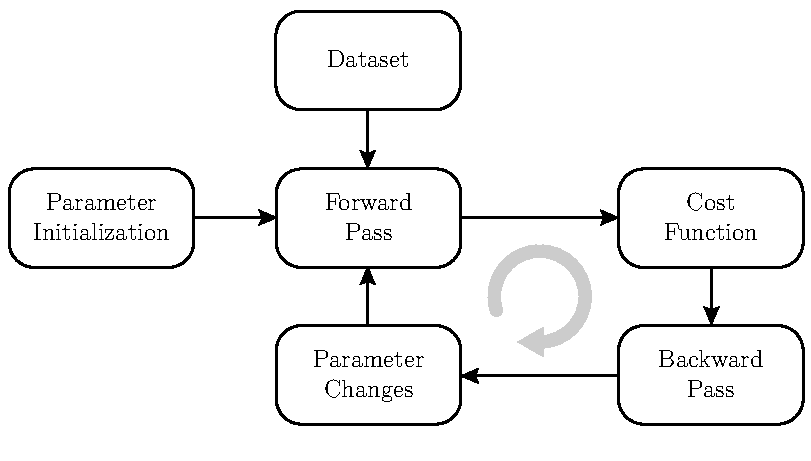
\includegraphics{images/training.pdf}
	\caption[Training process]{Training process}
	\label{fig:training}
\end{figure}

\input{tex/fundamentals/neural_networks/training/dataset}
\input{tex/fundamentals/neural_networks/training/weight_initialization}
\input{tex/fundamentals/neural_networks/training/forward_pass}
\input{tex/fundamentals/neural_networks/training/gradient_descent}
\input{tex/fundamentals/neural_networks/training/adam}
\subsection{Choice of Hyperparameters and Activations}
\label{sec:neural-networks-improving-performance}
Earlier sections make general recommendations on hyperparameters.
Finding well-suited ones is a trial-and-error method and requires much time.
However, there are methods that aim to find a good starting point.
Some of them are going to be presented in the following.

\input{tex/fundamentals/neural_networks/improving_performance/learning_rate.tex}
\input{tex/fundamentals/neural_networks/improving_performance/batch_size.tex}
\input{tex/fundamentals/neural_networks/improving_performance/activation_functions.tex}

\section{Software}
This section focuses on explaining which software and frameworks are used for implementing the network and generating the dataset.

\subsection{Tensorflow}
\label{sec:software-tensorflow}
Tensorflow is a free framework in particular for machine learning task.
It was originally developed by Google Brain for internal Google use and got finally licensed for open source. 
Mathematical operations are designed as a symbolic graph.
After its creation any operation inside can be executed and only needs the computation of its dependent operations.
Every computation involves tensors.
A tensor is a generalization of scalars, vectors and matrices independent on their dimension.
Hence, a definition of every tensor's size is important for a cost-effective creation and computation of the graph.
Due to the symbolic graph, it is possible to define a neural net with an input and output layer and steadily feed and compare different tensor values.
\subsection{Blender}
\label{sec:software-blender}
Blender is a free and open source 3D creation suite to model, texture and animate objects.
The integrated algorithms like lighting and shadowing offer default parameters that can be changed according to one's wishes.
Furthermore, it supports importing existing models and manipulating them.
Additionally, an API interface is provided, that can be used with the programming language Python, to control every function of Blender.
This eases repetitive tasks tremendously.

Every object in Blender has its own coordinate system.
Hence, a way of expressing points of one coordinate system in another would be useful.
Let's define a world coordinate system $\mathcal{W}$ with the origin $\vec{o}_\mathcal{W} = (0,0,0)^T$ and the rotation $\vec{r}_{\mathcal{W}} = (0,0,0)^T$, where each element of the latter represents a rotation around the $x$-, $y$- or $z$-axis, respectively, in radians.
This system contains every other system.
Now another coordinate system $\mathcal{L}$ is created, of course, inside the world coordinate system.
However, $\mathcal{L}$ can be translated and rotated in comparison to $\mathcal{W}$.
Hence, every coordinate system has a rotation matrix $\vec{R}$ in Euler representation and a translation vector $\vec{t}$ that stores how they are rotated and translated to every other coordinate system.
Considering $\mathcal{L}$ and $\mathcal{W}$ yields
\begin{align}
	\vec{R}_{\mathcal{L} \rightarrow \mathcal{W}} &= \vec{R}_{\mathcal{W} \rightarrow \mathcal{L}}^{-1} \\
	\vec{t}_{\mathcal{L} \rightarrow \mathcal{W}} &= - \vec{t}_{\mathcal{W} \rightarrow \mathcal{L}}
\end{align}
as properties, where the subscript indicates the transfer.
Transferring the coordinates of an arbitrary local point $\vec{x}_{\mathcal{L}}$ into corresponding coordinates $\vec{x}_{\mathcal{W}}$ of the reference coordinate system is done by using
\begin{equation}
	\vec{x}_{\mathcal{W}} = \vec{R}_{\mathcal{L} \rightarrow \mathcal{W}} \cdot \vec{x}_{\mathcal{L}} + \vec{t}_{\mathcal{L} \rightarrow \mathcal{W}}
\end{equation}
as the general expression.
\chapter{Methods}
\label{sec:methods}
This chapter explains the generation and preparation of the dataset and the implementation of the neural network architecture for classifying objects depending on their color feature.
The input consists of multiple views of an object, while percentages of class memberships are outputted.
The creation of the dataset is supported by the Blender API interface, while the model is written in Python using the tensorflow framework.

\section{Dataset Generation}
\label{sec:methods-dataset-generation}

\subsection{Choosing a Dataset}
\label{sec:dataset-choosing}
One requirement of the dataset is, that there are multiple views of the same object available.
Optimally, these views can be arbitrarily chosen for having as much freedom as possible for training and evaluating the network.
Hence, three-dimensional objects are necessary.
The related object categories are preferably discriminative to each other due to the objective of classifying real-world objects and easier evaluation of the model.
This means the dataset should not contain only flowers or faces for example.
These constraints bring up two possibilities.
The first one is creating new CAD objects.
These can be modeled in a way that supports the own needs the most.
However, creating plenty of models for every category would take a huge amount of time.
The second option is to use CAD models of an existing dataset.
Referring to the first possibility, this one just takes the time for finding a suited dataset and perhaps some slight modifications.
The time for manipulating this one according to the wanted color features compared to the self-created one is probably identical and, therefore, not taken into account.
Another advantage is the competitive ability because if this one is a popular dataset, other researches probably used it as a benchmark for their neural network as well.
Hence, a qualitative evaluation would be possible.
Taking all these arguments into account, an existing dataset is the best choice.

There are three different techniques for building a three-dimensional shape.
One uses triangles, where each one is defined by the position of its edges.
These positions are called vertices and contain an $x$-, $y$- and $z$-coordinate.
Additionally, each triangle has a normal vector and other information like a color and a texture.
Combining several triangles results in the final shape that is called a mesh object.
Another one uses voxels.
This word is a portmanteau of "volume" and "pixel" and represents a cell in a three-dimensional grid.
Each voxel behaves like a pixel and has a color.
The last technique is the point cloud.
Each point is represented by a vertex.
Such a cloud is often created by 3D scanners that measure a large number of points in a scene, like distances and sometimes color for digitalizing it.
A comparison of these techniques yields that the mesh object is the best-suited one.
It has the smoothest surface because it is continuous, hence, representing real-world objects most likely.
Using enough voxels could result in a similar shape, but the data size would be much bigger.
Furthermore, applying a color feature to a single triangle is easier than applying it to several voxels, where connected ones need to be found first.

The most popular dataset containing CAD objects in polygon mesh representation is ModelNet\cite{conf/cvpr/WuSKYZTX15}.
It contains 127,915 CAD models divided into 662 object categories for now.
For convenience, there are a 10-class and 40-class subset containing 10 or 40 popular categories, respectively.
Both are cleaned in respect to a wrong category sorting and then split into a training and a testing set.
Furthermore, the orientations of the models of the first one are aligned as well.
\subsection{Rendering Views of CAD Models}
\label{sec:dataset-rendering}
The following explains how multiple viewing perspectives of a single model are generated.
The properties of each CAD model of ModelNet are stored in a file that is loaded and interpreted in Blender.
To be able to refer to faces they are all part of the same basic coordinate system and are placed according to their defined vertices.
Because all models are oriented beforehand, their top points along the $z$-axis.
The origin of this coordinate system is set to the center of mass depending on the face areas.
For adding lighting to the object a lamp needs to be placed inside that coordinate system.
Blender offers several lamp types, but the Hemi lamp was chosen because it emits light radially from a plane.
Therefore, a homogeneous illumination is ensured.
%\begin{figure}
%	\centering
%	\begin{subfigure}{0.19\textwidth}
%		\centering
%		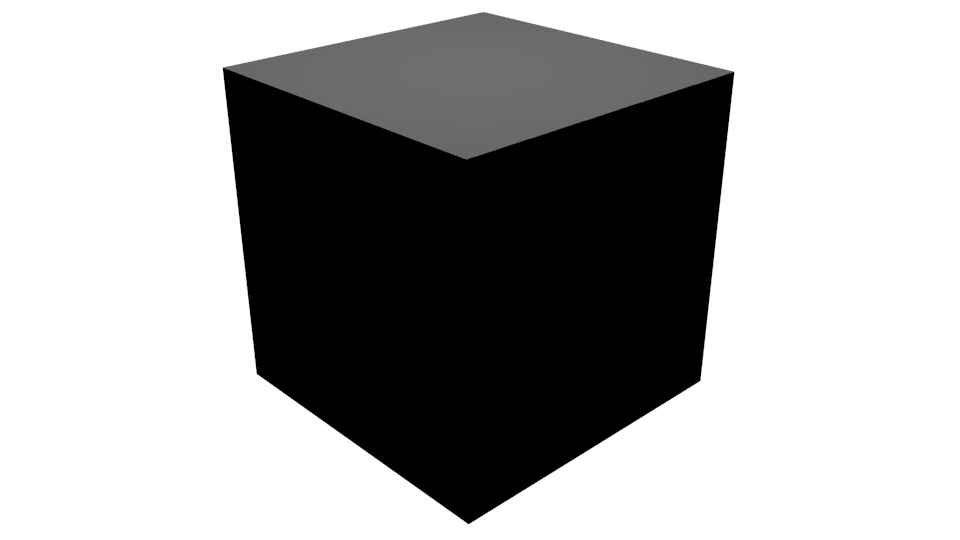
\includegraphics[width=\textwidth]{images/point.png}
%		\caption{Point}
%	\end{subfigure}
%	\begin{subfigure}{0.19\textwidth}
%		\centering
%		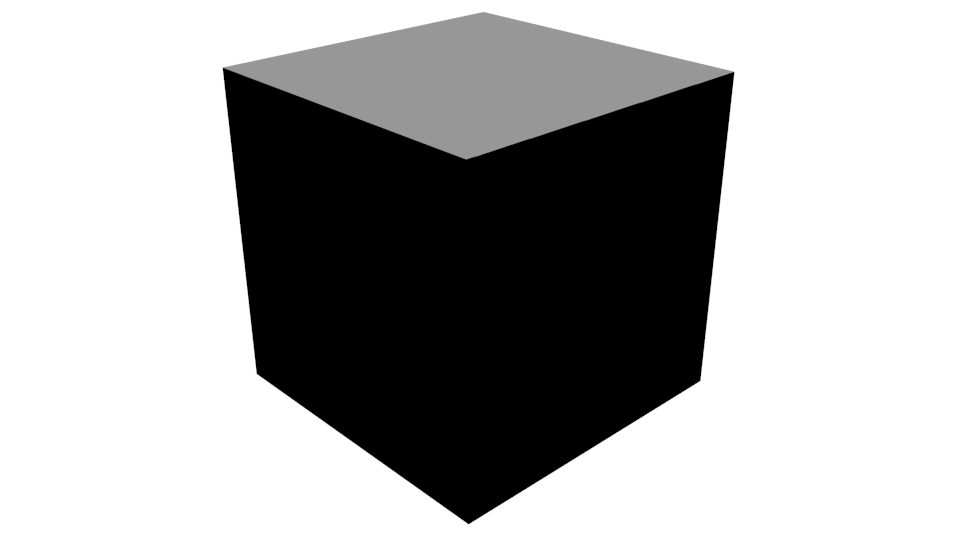
\includegraphics[width=\textwidth]{images/sun.png}
%		\caption{Sun}
%	\end{subfigure}
%	\begin{subfigure}{0.19\textwidth}
%		\centering
%		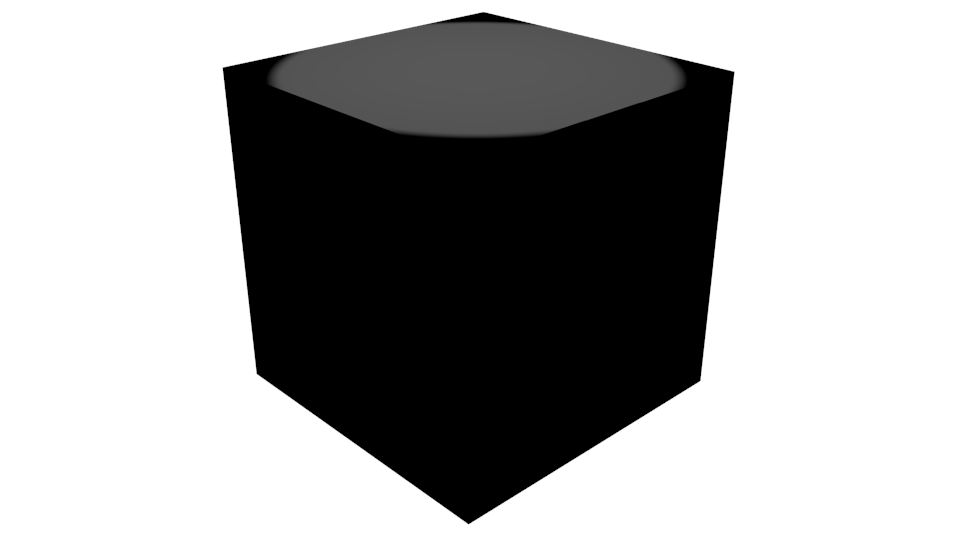
\includegraphics[width=\textwidth]{images/spot.png}
%		\caption{Spot}
%	\end{subfigure}
%	\begin{subfigure}{0.19\textwidth}
%		\centering
%		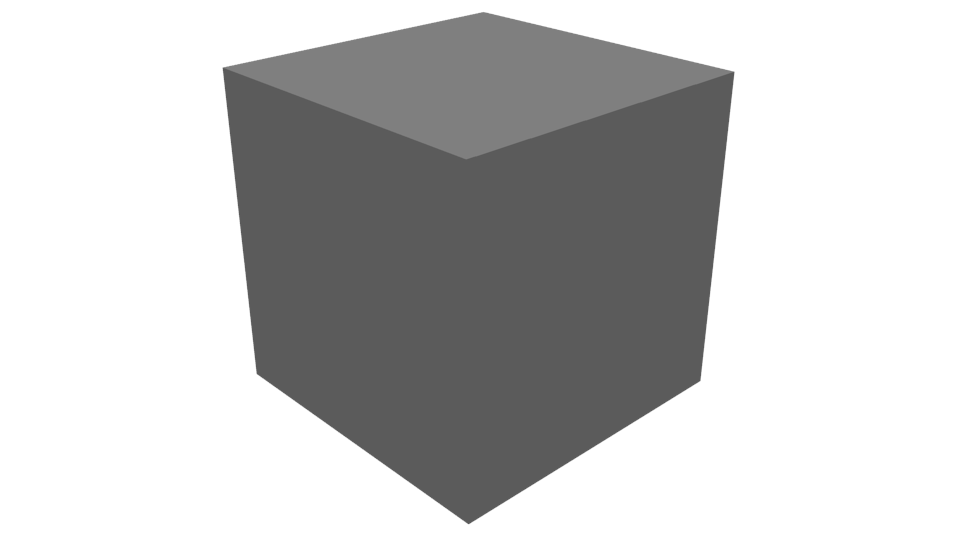
\includegraphics[width=\textwidth]{images/hemi.png}
%		\caption{Hemi}
%	\end{subfigure}
%	\begin{subfigure}{0.19\textwidth}
%		\centering
%		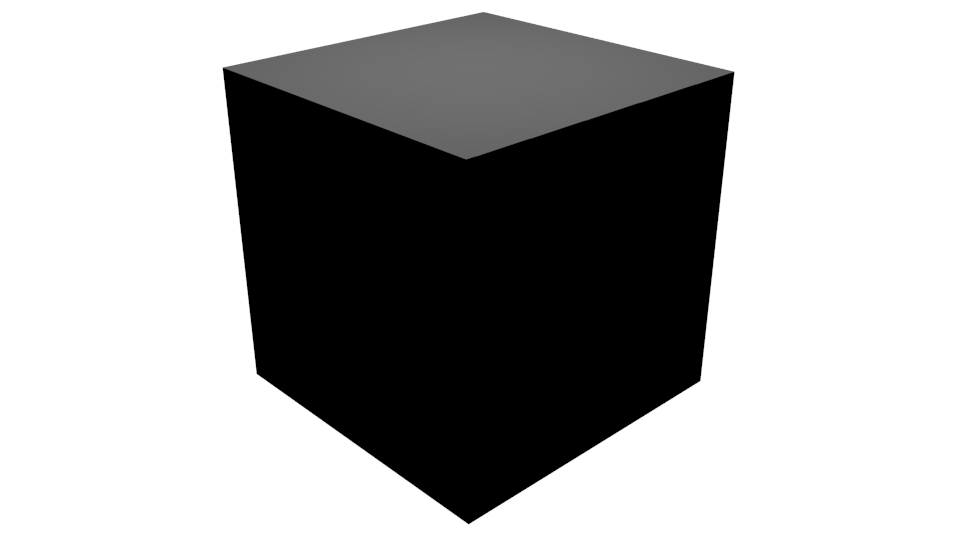
\includegraphics[width=\textwidth]{images/area.png}
%		\caption{Area}
%	\end{subfigure}
%	\caption[Lamp types available in Blender]{Lamp types available in Blender. Each light source is placed above the cube pointing directly towards it.}
%	\label{fig:blender-lamps}
%\end{figure}
Because all models have different heights and this type of lamp has no decay of intensity, it is placed above the objects far away from their origins.
By assigning the lamp a direction $\vec{r}_l = (0,0,0)^T$ it emits light along the negative $z$-axis directly onto the model.

For rendering views, a camera object is required.
Its parameters are left to the default values, except its view distance, which is set very high to work with all models.
Hence, only its location and rotation needs to be set.
Following the approach from \cite{Su:2015:MCN:2919332.2919750, Su2018} the camera is elevated 30 degrees from the ground plane and points towards the origin.
This results in the first rotation vector
\begin{equation}
	r_{c,0} = \left( \frac{r_{x,\text{deg}} \cdot \pi}{180}, 0, 0 \right)^T = \left( \frac{60 \cdot \pi}{180}, 0, 0 \right)^T
\end{equation}
in radians, where $r_{x,\text{deg}}$ is the rotation around the $x$-axis in degrees.
The first, second and third element define a rotation around the $x$-, $y$- and $z$-axis, respectively.
Because the camera points along the negative $z$-axis in its own coordinate system by default, $r_{x,\text{deg}} = 60$ corresponds to the mentioned setup.
The next step is fitting the camera view to the model just by changing the location of the camera.
Because Blender fits the camera view exactly to the object, an image padding is necessary for having empty border regions for later convolutions.
This is achieved by moving the camera away from the object along the line of their centers, i.\,e. along the negative view direction.
It is moved by
\begin{equation}
	\Delta d = \frac{d}{10}
\end{equation}
where $d$ is the distance from the mesh origin to the camera.
The advantage of a fraction is, that the padding is independent of the model's size.
Finally, this camera view is rendered with the following properties.
The resolution is defined to be $224 \times 224$ pixel
Furthermore, it needs to be coped with aliasing.
Because every pixel can only have a single color, diagonal lines usually have a step pattern.
This is not realistic, hence, it is smoothed out by anti-aliasing techniques.
This works by rendering the related image region in a higher resolution, taking several samples of pixel values and averaging them to get the value of the pixel in the desired resolution.
The best available sample size in Blender is 16, hence, it is chosen.
The background color is left at the default RGB color $\vec{c} = (64, 64, 64)$ resembling a dark gray for adding some noise to the views.
A black background would yield pixel intensities of 0 and resembles, in general, no real-world views.
Finally, this view is saved as a PNG file.
For gathering multiple views, the camera needs to be repositioned.
Hence, the following steps are repeated for the desired number of views.
The rotation of the camera is set to
\begin{equation}
	\vec{r}_c(v_i) = \left(  \frac{60 \cdot \pi}{180}, 0, \frac{v_i \cdot \varphi \cdot \pi}{180} \right)^T
\end{equation}
where $v_i$ is the view index, originally starting at 0, and $\varphi$ the moving interval in degrees.
The latter is set to
\begin{equation}
	\varphi = \frac{360}{n_v} = \frac{360}{12} = 30
\end{equation}
where $n_v$ equals the number of views.
For the ability to compare this work to related researches, $n_v = 12$ is defined.
The number of objects per set corresponds to \cite{Su:2015:MCN:2919332.2919750}.
That means, 90 objects per category class for the training set and 30 for the test set.
This process is repeated for each CAD object.
\subsection{Applying Material Feature Manipulations}
\label{sec:dataset-material-feature}
The objective is to clone every model and apply a color feature to every clone to be able to distinguish the same models.
Cloning is a trivial task because this can be done by rendering the native object first and then the color featured one.
One method for the color feature manipulation is preparing a color feature like a colored circle as an image and putting it on the model.
This feature can be scaled dependently on all the face areas for achieving a similar scale across all models.
However, clinging this image to a model considering all its edges is problematic.
It would be necessary to find a way to unfold the model along its edges.
This can be done by hand but is very time-consuming and complex.
In fact, Blender supports an automatic way of unfolding, but its results are not satisfying.
Therefore, this approach is not further pursued.
Another method is to color vertices.
However, for achieving reasonable features, a high number of vertices is necessary.
There is an option to subdivide existing faces and add additional vertices, but this increases the data size extremely, which needs much more computer performance and has the risk of inducing unwanted geometry into the model.
Hence, coloring single faces becomes the chosen approach due to its simplicity.
In CAD modeling objects are assigned a material with a color that reacts to light which produces shadows.
In Blender, the default material's color is a slightly darkened white.
Changing the color of a face is performed by changing the color of its material.

For following this approach, it is advisable to pre-define material presets.
Those presets consist of the default material but have different colors.
After making those presets available to the Blender scene, a well-suited face for being colored needs to be found.
In the following those faces are referred to as an optimal face.
It is important to filter all faces of an object by their area size.
\figref{fig:face-area-filter} shows why and the results of several thresholds.
\begin{figure}
	\centering
	\begin{subfigure}{.32\textwidth}
		\centering
		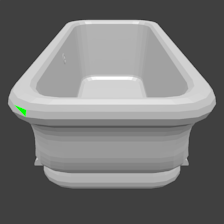
\includegraphics[width=\textwidth]{images/face_area_unfiltered.png}
		\caption{Unfiltered}
		\label{fig:face-area-unfiltered}
	\end{subfigure}
	\begin{subfigure}{.32\textwidth}
		\centering
		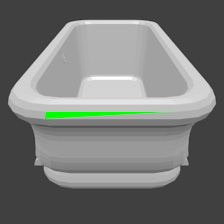
\includegraphics[width=\textwidth]{images/face_area_mean.png}
		\caption{Face Area Mean}
		\label{fig:face-area-mean}
	\end{subfigure}
	\begin{subfigure}{.32\textwidth}
		\centering
		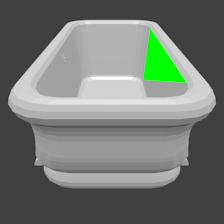
\includegraphics[width=\textwidth]{images/face_area_max_dependent.png}
		\caption{Max Face Area Dependent}
		\label{fig:face-area-max-dependent}
	\end{subfigure}
	\caption{Threshold setup for filtering faces by their area size}
	\label{fig:face-area-filter}
\end{figure}
If faces are not filtered at all, any face can result in being the optimal one.
However, it is not guaranteed that this face has a decent size and can be seen and recognized by the network easily.
This assumption was later verified by a not changing loss value during training.
Like in \figref{fig:face-area-unfiltered} the optimal face is comparatively small to the whole model.
Accepting only faces as the optimal face, that have at least the size of the mean of all faces lead to a result like in \figref{fig:face-area-mean}.
The optimal face can be seen more easily than before, but this threshold often results in long and slender optimal faces.
This is due to the fact, that the chosen object categories mostly contain objects that are built using such faces because they have longish surfaces.
Hence, filtering by the mean of the faces amplifies the probability to choose such a face as an optimal one.
Therefore, a threshold of above the mean is desired to skip all those lathy faces like it is shown in \figref{fig:face-area-max-dependent}.
Additionally, larger faces should be preferred.
Thus, the area of the optimal face have to satisfy
\begin{equation}
	\alpha_{\text{opt}} > (\alpha_{\text{mean}} + \alpha_{\text{max}}) \cdot \lambda
\end{equation}
where $\alpha$ are the related areas and $\lambda$ a scalar.
With $\lambda = 0.3$ satisfying results are achieved.

Furthermore, it needs to be guaranteed, that the optimal face is visible in at least one view and not visible in at least one view.
This is validated by casting rays from the camera center onto the possible optimal face for every camera position that was defined in \secref{sec:dataset-rendering}.
In brief, if the rays hit the face, the face is visible.
Fortunately, there is a function in Blender performing this approach and returning among others the index of the face that is hit.
However, this cannot be performed for every pixel of a face due to performance issues.
Thus, the trade-off against accuracy is only checking the vertices defining the face.
This can raise errors, though, because a vertex can define multiple faces and it is not certain which face index the function returns.
Hence, each checkpoint $\vec{p}_i$ is moved slightly to the center of the face $\mathbb{F} = (v_{f1}, v_{f2}, v_{f3})$ by
\begin{equation}
	\vec{p}_{fi} = \vec{v}_{fi} + 0.05 \cdot (\vec{f}_o - \vec{v}_{fi})
\end{equation}
where $\vec{v}_{fi}$ is the related vertex and $\vec{f}_o$ the center of the face.
If the ray cast is valid for at least one checkpoint the face is supposed to be visible.
If all rays hit the wrong face, the current face is supposed to be not visible.
As soon as both conditions are satisfied for the examined face among all views, it becomes the optimal face.
Otherwise, the next possible face is investigated.
If the conditions are never satisfied for each possible face, the object is skipped at all.

It is found, that a single optimal face is not enough, because some models have several duplicated faces.
Those are different faces where the coordinates of all the describing vertices are identical to the ones of other faces.
Hence, there are faces laying into each other.
This results in rendering issues like it is shown in \figref{fig:optimal-face}, because the rendering engine does not know, which material should be rendered on the surface.
In \figref{fig:optimal-face-single} only one of two identical faces is colored, which leads to the noticeable transparency effect.
That is one of the brighter effects, though.
It is also possible that one optimal face is shown normally and only on the edge rendering issues are visible like a dotted line with the colors of all optimal faces. 
Nevertheless, any of these effects could induce false correlations into the dataset that are not available on real-world objects, hence, leading to a not practical network.
Thus, in \figref{fig:optimal-face-all} the materials of all identical faces are changed, which leads to realistic color representations.
\begin{figure}
	\centering
	\begin{subfigure}{.49\textwidth}
		\centering
		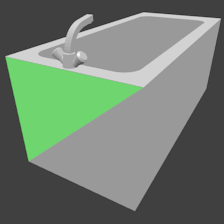
\includegraphics[width=.7\textwidth]{images/optimal_face_single.png}
		\caption{Single Optimal Face}
		\label{fig:optimal-face-single}
	\end{subfigure}
	\begin{subfigure}{.49\textwidth}
		\centering
		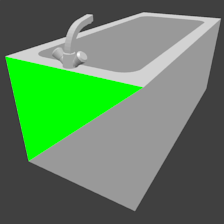
\includegraphics[width=.7\textwidth]{images/optimal_face_all.png}
		\caption{All Optimal Faces}
		\label{fig:optimal-face-all}
	\end{subfigure}
	\caption{Material manipulation on duplicated optimal faces}
	\label{fig:optimal-face}
\end{figure}

Regarding a validation of the later model, an examination of two material features per object would be interesting.
Hence, for applying another material change on a model, another optimal face or faces, respectively, needs to be found.
A requirement for this is the presence of only one material feature in a single view.
Due to the automation of this task, a reliable solution is necessary.
One approach would be using the other side of the surface of the first optimal face.
However, this fails if the surface has a thickness of more than a single face.
Then the next face along its normal needs to be found by ray casting and then the visibility of this face needs to be verified.
Thus, this process leads to excessive ray cast validations and therefore not followed up on.
However, it is considered, that faces at a similar location as the original optimal face are well-suited as well.
Thus, the choices of further optimal faces are narrowed down by sorting all remaining faces by their distance from their center to the center of the first optimal face in descending order.
The intention is that choosing faces with the largest distances result in either a kind of opposite face or in a face that is that far away to not be visible at the same time. as the first optimal face.
Of course, the tasks of checking the visibility and finding identical faces are performed on the new face as well.
If no additional optimal face is found, the model is skipped, although, this never happened during execution.
\section{Preparing the Dataset}
\label{sec:methods-prepare-data}

\subsection{Single-View to Multi-View Conversion}
\label{sec:prepare-data-view-conversion}
The views created in \secref{sec:dataset-material-feature} exist in a single view representation.
Thus, a multi-view classification should be performed by the network.
This means, each input represents a model with all its corresponding views.
Hence, each model's single views need to be converted into a related multi-view representation.
For achieving this the single views needs to be collected first.
From a given custom file path to the dataset all model views are collected recursively in a sorted order.
This is necessary for keeping related views in the order by which they are created.
Due to the self-explanatory folder structure, models for the training and testing set can be handled independently.
To each of the sets belongs a list $\vec{\tilde{X}}_{set}$ for storing all related views in RGB color representation.
Now, each view's pixel values are read, normalized to a range between 0 and 1 and then stored in a matrix or array $\vec{X}_{set}^{(i)}$, respectively, which is added to one of the just mentioned lists.
Simultaneously to the view gathering each label needs to be created as well and put into a list $\vec{\tilde{Y}}_{set}$ similar to the views.
Getting the category is quite simple, because the file path of the view is known.
Hence, the second to last element of the view's file path represents the category label.
The file name of a view is build like \textit{category\_object-id\_material-id\_view-id.ext}.
Here is the material index label extracted by splitting the file name by "\textit{\_}" first and then taking the third split element.
Depending on the classification task of the model, those two labels possibly need to be combined.
The single-label classification case embraces the following configurations.
If categories and materials are classified, both labels are appended to each other.
This results in $n_l = n_c \cdot n_m$ labels, where $n_c$ is the number of categories and $n_m$ the number of materials.
If only categories or materials are classified, the final label is the category label or the material label, respectively.
Logically, the number of labels is either $n_l = n_c$ or $n_l = n_m$.
In the multi-label classification case both labels are used independently.
Hence, the number of labels equals $n_l = n_c + n_m$.
An example of those configurations is shown in \tabref{tab:label-generation}.
\begin{table}[]
	\centering
	\caption[Label Generation]{Label Generation with example categories "bathtub" and "sofa" and materials "0" and "1" for different cases of classifications.}
	\label{tab:label-generation}
	\begin{tabular}{l|l|l}
		Classification      & Single-Label                                                                        & Multi-Label                                                    \\ \hline
		Category + Material & \begin{tabular}[c]{@{}l@{}}bathtub\_0\\ bathtub\_1\\ sofa\_0\\ sofa\_1\end{tabular} & \begin{tabular}[c]{@{}l@{}}bathtub\\ sofa\\ 0\\ 1\end{tabular} \\ \hline
		Category            & \begin{tabular}[c]{@{}l@{}}bathtub\\ sofa\end{tabular}                              & n/a                                                            \\ \hline
		Material            & \begin{tabular}[c]{@{}l@{}}0\\ 1\end{tabular}                                       & n/a                                                           
	\end{tabular}
\end{table}
When the number of labels is known, a one-hot encoding is performed on each label.
In conclusion, this process results in four lists
\begin{subequations}
	\begin{align}
		\label{eq:list-x-train}
		\vec{\tilde{X}}_{train} &=
		\begin{pmatrix}
			\vec{X}_{train}^{(1)} & \vec{X}_{train}^{(2)} & \cdots & \vec{X}_{train}^{(m_{train})}
		\end{pmatrix}
		\\
		\label{eq:list-x-test}
		\vec{\tilde{X}}_{test} &=
		\begin{pmatrix}
			\vec{X}_{test}^{(1)} & \vec{X}_{test}^{(2)} & \cdots & \vec{X}_{test}^{(m_{test})}
		\end{pmatrix}
		\\
		\label{eq:list-y-train}
		\vec{\tilde{Y}}_{train} &=
		\begin{pmatrix}
			\vec{y}_{train}^{(1)} & \vec{y}_{train}^{(2)} & \cdots & \vec{y}_{train}^{(m_{train})}
		\end{pmatrix}
		\\
		\label{eq:list-y-test}
		\vec{\tilde{Y}}_{test} &=
		\begin{pmatrix}
			\vec{y}_{test}^{(1)} & \vec{y}_{test}^{(2)} & \cdots & \vec{y}_{test}^{(m_{test})}
		\end{pmatrix}
	\end{align}
\end{subequations}
where $\vec{X}^{(i)}$ and $\vec{Y}^{(i)}$ of the same set are building an input-output pair.

Those single view and label representations need to be converted to a multi-view representation.
Because sorted data was read in, it is known that each 12 elements belong together and need to put together somehow.
Looking at common definitions yields, that images are a three-dimensional matrix with the shape definition $Height \times Width \times Channels$.
Furthermore, Tensorflow mostly uses the shape definition $Batch \times Height \times Width \times Channels$ for tensors.
Hence, assuming each view as a batch element is a reasonable approach.
If an actual batch dimension becomes necessary it is inserted as a new first dimension.
This yields a reduction of \thmref{eq:list-x-train} and \thmref{eq:list-x-test} to a $n_v$-th of its size, where $n_v$ is the number of views.
The labels can be processed similar, however, much easier.
Because each $n_v$ labels are identical, it is sufficient to just keep every $n_v$-th label.
For a later lookup of the labels they are saved to the disk as a text file.
\section{Multi-View Network Architecture}
\label{sec:methods-architecture}
Because convolutional neural networks are well-suited for image classification task, this approach is pursued.
Furthermore, in \cite{Su:2015:MCN:2919332.2919750} the VGG-M\cite{journals/corr/ChatfieldSVZ14} architecture is used and in \cite{Feng2018} GoogLeNet\cite{szegedy2015}.
Both are convolutional neural networks, where the first uses 8 layers and the latter, that is more recent, 22, however, both of them yield satisfying results.
The number of parameters of both is too large for the available resources for this work, though.
Hence, the AlexNet architecture\cite{Krizhevsky:2012:ICD:2999134.2999257} is chosen.
It is very similar to the VGG-M one, but uses larger filters for convolutions and less nodes in the fully connected layers.
However, the lesser parameters are a trade-off for accuracy.

In \cite{Feng2018} it is shown that the performance of the network from \cite{Su:2015:MCN:2919332.2919750} can be improved even more by grouping views with similar informational content and giving their descriptors more weight during the classification.
It is supposed that in particular the grouping process suits the task of distinguishing same models with different materials very well.
Because the material is the only difference, the related views should be weighted the most while all others should only play a marginal role in the classification process.
This would reduce noise and thus results in a better performance.
Hence, the network is divided into three important modules as illustrated in \figref{fig:architecture-modules}.
The feature module takes all views of an object and calculates a descriptor for each.
Those are fed to the grouping module, that groups views dependent on their information content and generates a descriptor for every group and additionally their weight.
Dependent on those outputs a single descriptor is calculated, that describes the inputted shape or object, respectively, and is used for the classification.
Each of the modules is examined in detail in the following sections.
\begin{figure}
	\centering
	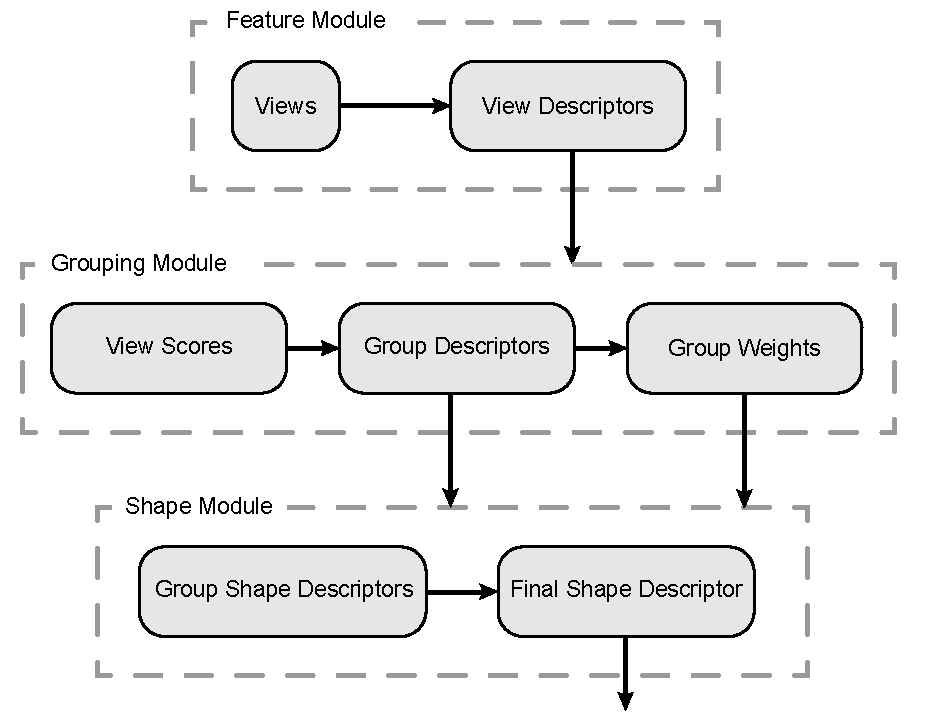
\includegraphics[]{images/multi_view_architecture.pdf}
	\caption{Modules of the Multi-View Architecture}
	\label{fig:architecture-modules}
\end{figure}

\subsection{Feature Module: Generating View Descriptors}
\label{sec:architecture-feature-module}
The objective of the feature module is the generation of a descriptor for each view $v$ by using five convolutional layers.
Each one is referred to as a view descriptor $\vec{V}^{[l]}_v$ of the $l$-th layer in the following.
\figref{fig:feature-module} shows the basic concept.
\begin{figure}
	\centering
	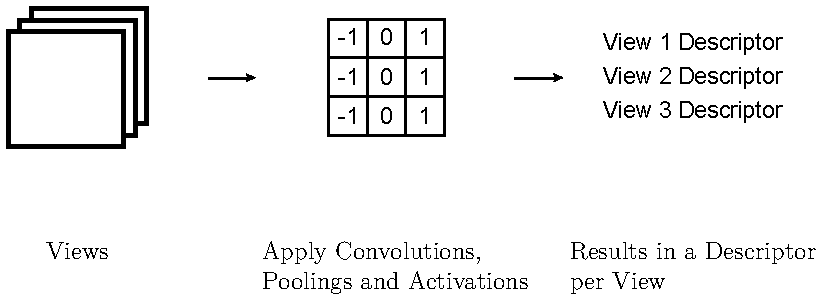
\includegraphics[]{images/feature_module.pdf}
	\caption{Basic concept of the feature module. On each view $v$ of a multi-view $\tilde{\vec{X}}^{(i)}$ of the $i$-th sample convolutions and poolings are performed yielding the final view descriptors $\vec{V}^{[5]}_v$.}
	\label{fig:feature-module}
\end{figure}
This module is the first one in the feed-forward chain.
Its input is a multi-view $\tilde{\vec{X}}^{(i)}$ of the $i$-th object.
Because tensorflow supports batch execution, i.\,e. all its operations can be applied to a batch of data, the multi-view input is converted to a tensor with a batch dimension for multiple multi-views.
This yields an input tensor of shape $Batch \times Views \times Height \times Width \times Channels$.
In the following, if a tensor has a batch dimension, which is usually the case, it is assumed that any mentioned operation or approach is applied to every batch element.
This module consists of five main convolutional layers.
A main convolutional layer consists of a convolutional layer and an optional pooling layer.
The first main layer performs a valid convolution with 96 filters $\vec{K}^{[1]}$ of size $7 \times 7$ and a stride of $s=2$ on each $224 \times 224 \times 3$ multi-view view.
Every filter extracts different features.
In comparison, the original AlexNet uses filters $\vec{K}^{[1]}$ of size $11 \times 11$ and a stride of $s=4$.
However, it is assumed that smaller filters and a smaller stride are collecting more information that can be used for a classification of the object and material at once.
A convolution operation is performed by moving a filter across a input and calculating each dot product.
This results in the view descriptor $\vec{V}^{[1]}$ with a size of $Views \times 109 \times 109 \times 96$ in this case.
Furthermore, to each convolution output, the corresponding bias is added.
This result is fed into a ReLU activation function.
Finally, the outputs are max-pooled with a window $\vec{K}_{\text{max}}$ of size $3 \times 3$ and a stride of $s=2$.
No padding is applied.
It is defined, that the max-pooling is always performed on the last dimension, i.\,e. the one containing each feature.
This yields a matrix of shape $Views \times 54 \times 54 \times 96$ for each pooling in the first main convolutional layer.
For simplicity, it is defined that within each main layer the view descriptor is reused.
Hence, the output of the $l$-th main layer is the view descriptor $\vec{V}^{[l]}$.
The next layers are similar including the bias addition and the ReLU activation function.
Hence, only the operations and their parameters will be mentioned.
Furthermore, the layers are added sequentially.
That means, the activations of the previous main layer are the input of the current main layer and so on.
The second main layer performs a convolution with 256 filters $\vec{K}^{[2]}$ of size $5 \times 5$ and a stride of $s=2$.
However, this time the input is padded in a way, that the output has the original input's size.
This yields a convolution result $\vec{V}^{[2]}$ of shape $Views \times 27 \times 27 \times 256$.
The max-pooling uses again a window $\vec{K}_{\text{max}}$ of $3 \times 3$ and a stride of $s=2$.
The valid padding technique is applied resulting in a shape of $Views \times 13 \times 13 \times 256$.
The third and fourth main layer use 384 filters $\vec{K}^{[3]}$ and $\vec{K}^{[4]}$ of size $3 \times 3$ for the convolution task with a stride of $s=1$ each and the padding technique same.
However, no pooling is performed.
Hence, this yields a matrix $\vec{V}^{[3]}$ and $\vec{V}^{[4]}$ of shape $Views \times 13 \times 13 \times 384$ both the times.
For the last main layer, the fifth one, a convolution with 256 filters $\vec{K}^{[5]}$ of size $3 \times 3$ is performed.
The stride is $s=1$ and the padding technique same, hence, the result $\vec{V}^{[5]}$ has a size of $Views \times 13 \times 13 \times 256$.
The output's dimension is reduced with a valid max-pooling $\vec{K}_{\text{max}}$ of size $3 \times 3$ and stride $s=2$ to $Views \times 6 \times 6 \times 256$.
In the end, this whole process results in a tensor $\bar{\vec{V}}^{[5]}$ containing each view's view descriptor $\vec{V}^{[5]}$ of size $Views \times 6 \times 6 \times 256$ of every batch element.
Hence, this tensor's shape is $Batch \times Views \times 6 \times 6 \times 256$.
\subsection{Grouping Module: Generating Group Descriptors}
\label{sec:architecture-grouping-module}
The objective of the grouping module is grouping several view descriptors of an object depending on their information content.
The view descriptors $\vec{V}^{[5]}_v$ of each group $\mathbb{G}_g$ are then combined to a group descriptor $\vec{G}_g$.
Hence, the module's input are the view descriptors coming from the feature module.
\begin{figure}
	\centering
	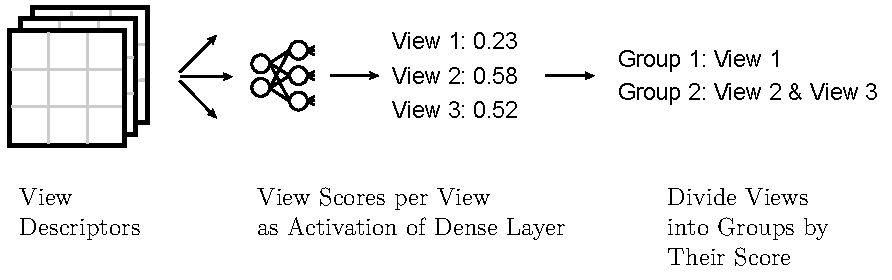
\includegraphics[]{images/grouping_module_groups.pdf}
	\caption{Group creation and view sorting in grouping module}
	\label{fig:grouping-module-groups}
\end{figure}
First, the informational content of each view needs to be calculated.
The simplest and most intuitive way is to give every view a single number representing its score of discrimination.
One approach would be to make the score directly depend on the pixel values.
This could be performed with a fully-connected layer with the pixels as inputs and the score as output.
However, like with fully-connected neural networks, this leads to a stiffness of the network due to its translation-variance of input values. 
This could be overcome by using convolutions first for extracting features.
However, such features are already extracted, presumably much more accurate than a few convolutions for the score would do. 
Hence, the followed approach is that each view's score depends on its latest descriptor.
It is worth noting, that in \cite{Feng2018} the view scores do not depend on the last convolution.
However, their network architecture uses more than five convolutional layers, but their scores depend on the fifth one.
This is probably because later features are too detailed and would result in too divergent discrimination scores for a reliable group generation.
Each latest view descriptor is fed into the same single fully-connected layer with 1 node.
Therefore, the view descriptor matrix is flattened into a row-wise vector, which is multiplied with the corresponding weight matrix $\vec{W}^{[d4]}$ of shape $6 \cdot 6 \cdot 256 \times 1$.
This results in a single value to which a bias $b^{[d4]}$ is added.
A dropout is not performed, because with only one node it is not desirable.
Dropping out this node represents a view discrimination score of 0.
Of course, this would generalize the view score, but a kind of overfitting on detailed features is desirable for evaluating views.
It is supposed that those discriminative features are reoccurring in different views if the latter is actually discriminative.
Thus, the more discriminative features a view has, the more discriminative it is.
Hence, they should be kept and used for training.
Finally, the weighted sum of a node is fed into its activation function.
It was found during training, that the unit died at the beginning of the training most of the time when using ReLU activation functions.
This is due to its characteristic.
If the weighted sum is zero or below at the beginning of the training due to an unsuited weight initialization, the activation is zero, hence, the neuron dies immediately.
Another reason could be a too large learning rate, allowing the weights to update in too big steps leading to a weighted sum of 0 or below.
This results in a view score of $0$ for every view that is not changed during later training steps due to a gradient of 0.
The learning rate should suit the whole network and not only this layer, though.
So, in contrast to every other layer in this network, leaky ReLU activation functions are applied to those units.
Their gradient is always unequal to zero, hence, it is solving the dying ReLU unit problem.

For interpretation purposes, the activation is squeezed into a range from 0 to 1 using the sigmoid function according to \cite{Feng2018} representing a probability of discrimination.
Because the sigmoid function saturates at values higher than around $\abs{5}$, but the activation of the fully-connected layer is assumed to be larger, the natural logarithm of the activation is computed first.
This shifts the saturation to values that are presumably not in the range of the activation.
For having a continuous function the absolute value of the activation is taken beforehand.
This yields the expression for a view's score
\begin{equation}
	\label{eq:view-discrimination-score}
	\theta = \sigmoid\left( \log \left( \abs{a^{[d4]}} + \varepsilon \right) \right)
\end{equation}
where $a^{[d4]}$ is the output or activation, respectively, of the fully-connected layer.
The small constant $\varepsilon=10^{-6}$ is added for numerical stability for avoiding $\log(0)$.
A plot of this function is shown in \figref{fig:view-discrimination-score}.
\begin{figure}
	\setlength\figureheight{.45\textwidth}
	\setlength\figurewidth{.8\textwidth}
	\centering
	\input{images/view_discrimination_score.tikz}
	\caption{View discrimination score function plot}
	\label{fig:view-discrimination-score}
\end{figure}
All view discrimination scores for a batch are stored in a tensor $\bar{\vec{\Theta}}$ with shape $Batch \times Views$.

Dependent on each view score, the related views are divided into groups.
For maximum flexibility, the number of groups $n_g$ equals the number of views $n_v$.
Hence, the size of each group $r_g$ is related to the number of views $n_v$ per object and the range of possible view scores $r_\theta$.
With the limit of \eqref{eq:view-discrimination-score}
\begin{equation}
	\lim_{x\rightarrow \infty} \sigmoid\left( \log \left( \abs{a^{[d4]}} + \varepsilon \right) \right) = 1
\end{equation}
and only positive values from the ReLU, scores are in the range $r_\theta = 1 - 0 = 1$.
Dividing $r_\theta$ in equal sized parts yields
\begin{equation}
	r_g = \frac{r_\theta}{n_v} = \frac{1}{12} \approx 0.083
\end{equation}
as each group's size.
Hence, a group $\mathbb{G}_g$ contains views with scores of $(g-1) \cdot r_g \leq \theta < g \cdot r_\theta$ where $g = {1,2, \dots, n_v}$.
\figref{fig:grouping-module-groups} illustrates the basic view score calculation and group dividing.
This example assumes a group size of $0.33$.
The group to which each view $\tilde{\vec{X}}^{(i)}_v$ belongs is calculated by
\begin{equation}
	g = \floor \left( \frac{\vec{\theta}_v}{r_g} \right)
\end{equation}
yielding the group's index, where $\vec{\theta}_v$ is the view score of the $v$-th view of the corresponding multi-view sample.
Those are stored for every view resulting in the group index vector $\vec{g}_{\text{idx}} = \left( g_1, g_2, \cdots, g_{n_v}\right)^T$.
The subscripts correspond to the view indices, e.g. $g_2$ belongs to $\tilde{\vec{X}}^{(i)}_2$.
With this approach, it is possible for groups to remain empty.
Based on the group indices, related view descriptors are averaged across their first dimension.
This means every channel of one view descriptor is averaged element-wise with the corresponding channel of the other view descriptors.
In brief, every feature is averaged.
This is illustrated in \figref{fig:grouping-module-group-descriptors}.
\begin{figure}
	\centering
	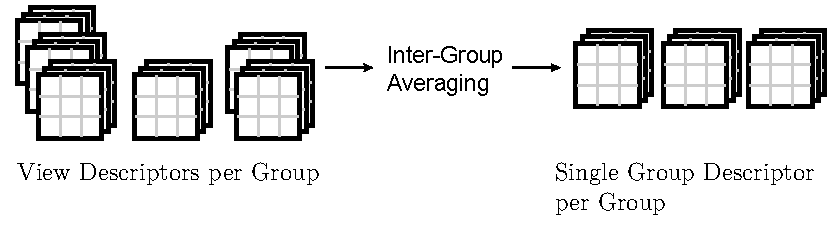
\includegraphics[]{images/grouping_module_group_descriptors.pdf}
	\caption[Generating group descriptors]{Generating group descriptors by calculating the average of related features.}
	\label{fig:grouping-module-group-descriptors}
\end{figure}
A normal average is chosen, because all views in a group should have similar extracted features, e.g. the left and right side of a car.
If the maximum of all features were taken, the group would presumably contain all views where important features were extracted for creating a group descriptor containing as many features as possible.
However, this is not desirable for the use case.
This results in a group descriptor
\begin{equation}
	\vec{G}_g = \frac{\sum_{\vec{D} \in \mathbb{G}_g} \vec{D}}{|\mathbb{G}_g|}
\end{equation}
with the same size as a view descriptor, where $\vec{D}$ is a view descriptor $\vec{V}^{[5]}$ of group $\mathbb{G}_g$. The addition and division are calculated element-wise.
However, the views of different objects are not necessarily divided into the same number of groups, thus, leading to a different number of group descriptors.
Due to tensorflow's constraint, that a tensor is not allowed to change its shape in a graph during execution, additional empty group descriptors need to be created for reaching the maximum possible number of group descriptors of $n_v$.
So, the final shape of the tensor $\bar{\vec{G}}$ containing all group descriptors is $Batch \times n_v \times 6 \times 6 \times 256$.

Every group $\vec{G}_g$ gets a weight $w_g$ assigned representing its discrimination.
This depends on the scores of its contained views.
Analog to before, views of a group are found by checking the group index vector $\vec{g}$.
This time the related view scores are summed up and divided by their number for calculating a mean.
In mathematical terms,
\begin{equation}
	{w}_G = \frac{\sum_{\vec{V} \in \mathbb{G}_g} \theta(\vec{V})}{|\mathbb{G}_g|}
\end{equation}
calculates the weight of the $g$-th group, where $\theta(\vec{V})$ is the score of a view $\vec{V}$ in $\mathbb{G}_g$.
Furthermore, the weight of a group is normalized by
\begin{equation}
	w_g = \frac{\hat{w}_g}{\max(\theta(\mathbb{G}_g))}
\end{equation}
to a range of 0 and 1, where $\max(\theta(\mathbb{G}_g))$ yields the maximum score of the given group, for being able to compare it with the ones in \cite{Feng2018}.
The calculation of the group weights is illustrated in \figref{fig:grouping-module-weights} referring to the example in \figref{fig:grouping-module-groups}.
\begin{figure}
	\centering
	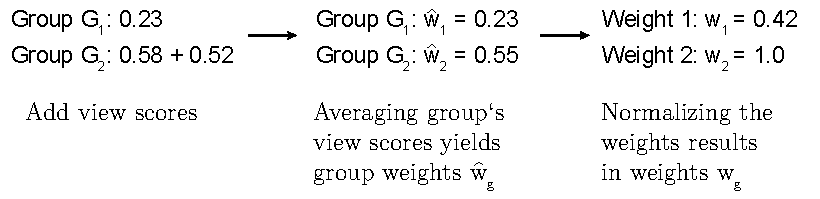
\includegraphics[]{images/grouping_module_weights.pdf}
	\caption{Calculation of group weights in grouping module}
	\label{fig:grouping-module-weights}
\end{figure}
The weights of the padded group descriptors equal 0 for being ignored in a later matrix multiplication.
Hence, the shape of the tensor $\bar{\vec{W}}_G$ storing all group weights is $Batch \times n_v$.
\subsection{Shape Module: Generating a Shape Descriptor}
\label{sec:architecture-shape-module}
The objective of the shape module is combining the group descriptors to a single shape descriptor that can be used for the classification.
This descriptor contains every important feature of all views and groups.
As usual, the tensor $\bar{\vec{G}}$ containing all the group descriptors of every batch is processed by each batch element.
This batch element $\vec{G}$ of size $n_v \times 6 \times 6 \times 256$ contains the $n_v$ group descriptors of an object.
This tensor is split across its first dimension, i.d. across the group descriptors, resulting in a tensor for each group descriptor.
Each group descriptor is then fed into a fully-connected sub-network with two layers.
The first layer has $6\cdot6\cdot256$ edges per unit and 4096 units in total, while the second layer has 4069 edges per unit and 4069 output units as well.
The inputs are processed like in the fully-connected layer before.
First, each input $\vec{G}_i$ is flattened into a row-vector $\vec{g}_i$.
Then, a matrix multiplication of the inputs and the corresponding weight matrix is performed and a bias vector is added.
This result is fed into a ReLU activation function $\phi(\cdot)$ resulting in an activation for the particular layer.
In conclusion, the two fully-connected operations
\begin{subequations}
	\begin{align}
		\vec{a}^{[d1]}_i &= \phi(\vec{g}_i \vec{W}^{[d1]} + \vec{b}^{[d1]}) \\
		\vec{a}^{[d2]}_i &= \phi(\vec{a}^{[d1]}_i \vec{W}^{[d2]} + \vec{b}^{[d1]})
	\end{align}
\end{subequations}
are performed as illustrated in \figref{fig:shape-module-group-shape}.
\begin{figure}
	\centering
	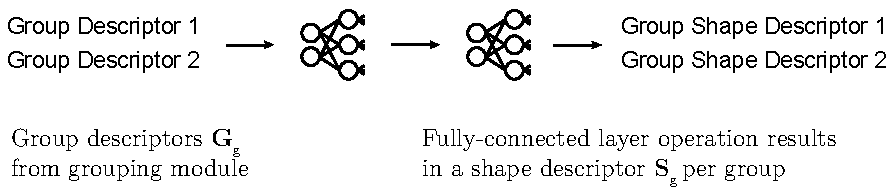
\includegraphics[]{images/shape_module_group_shape.pdf}
	\caption[Generate Group Shape Descriptors in Shape Module]{Generate Group Shape Descriptors in Shape Module. Each group descriptor is fed into two fully-connected layers representing layer 6 and 7 of the network. The activation of layer 7 represents the shape descriptor of each group descriptor.}
	\label{fig:shape-module-group-shape}
\end{figure}
Furthermore, both layers contain a dropout layer with a dropout probability of $0.5$.
This corresponds to the original AlexNet configuration.
Hence, the final activations of the seventh layer in the network or second dense layer, respectively, represent the shape descriptor of every group descriptor.
Those single shape descriptor vectors of each group are then again stacked along the first dimension for having a compact representation $\vec{S}_G$ with size $n_v \times 4096$.
Expanding this with a batch dimension yields the tensor $\bar{\vec{S}_G}$ with size $Batch \times n_v \times 4096$.

Now the group shape descriptors need to be combined for generating the final single shape descriptor of the object.
This is done by considering the group weights $\vec{w}$ with $n_v$ elements calculated in the grouping module.
As a reminder, they are the mean of all view scores of each group and, thus, an indicator for the group's discrimination.
Hence, a weighted average is calculated for considering this relation.
For having a valid matrix multiplication, the group shape descriptor $\bar{\vec{S}_G}$ needs to be transposed while keeping the batch dimension as the first one.
Hence its size changes from $Batch \times n_v \times 4096$ to $Batch \times 4096 \times n_v$.
Furthermore, the group weights tensor $\bar{\vec{W}}$ is expanded with a third dimension yielding the shape $Batch \times n_v \times 1$.
For this weighted average calculation a tensor holding the sums of the weights in inevitable.
Thus, $\bar{\vec{W}}_{sum}$ stores the sum of the group weights tensor along its first dimension, i.e. each element is the sum of all group weights of an object.
For a valid matrix division, a third dimension must be expanded as well.
This yields a tensor $\bar{\vec{W}}_{sum}$ of the shape $Batch \times 1 \times 1$ with weight sums.
Now the weighted average can be computed by
\begin{equation}
	\bar{\vec{S}} = \frac{\bar{\vec{S}_G} \bar{\vec{W}}}{\bar{\vec{W}}_{sum}}
\end{equation}
where the division is performed element-wise.
Due to the matrix multiplication, the padded entries have no impact.
The result has a shape of $Batch \times 4096 \times 1$ and represents the final single shape descriptor.
This can be made more compact by changing the shape to $Batch \times 4096$ without losing any information because the number of elements stays the same.

This representation is directly compatible with the last fully-connected layer, which is responsible for calculating the predictions of the network, thus, $\bar{\vec{S}}$ is fed into it.
The number of neurons in this layer equals the number of different labels or categories, respectively, where each neuron has 4096 edges.
The performed operations are identical to the ones earlier and are described by
\begin{equation}
	\vec{z}^{[d3]} = \bar{\vec{S}} \vec{W}^{[d3]} + \vec{b}^{[d3]}
\end{equation}
using the related weights and biases.
However, no activation function is applied here.
For making the predictions $\vec{z}^{[d3]}$ interpretable, they are fed into a softmax layer.
This outputs a valid probability distribution $\hat{\vec{y}}$ depending on all its inputs $\vec{z}^{[d3]}$.
Hence, this results in a membership probability for the network's input to each class.
The class representing the index with the largest value in $\hat{\vec{y}}$ is considered the predicted class. The functionality of the shape module is summarized in \figref{fig:shape-module-final-shape}.
\begin{figure}
	\centering
	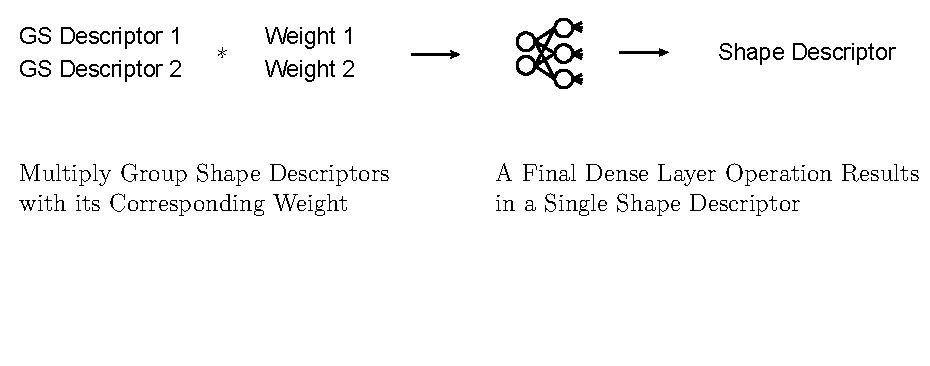
\includegraphics[]{images/shape_module_final_shape.pdf}
	\caption[Basic Concept of the Shape Module]{Basic Concept of the Shape Module Combined with a Classification. A weighted average of the group shape descriptors with the related group weights is calculated yielding a single shape descriptor. It is fed into the last fully-connected layer resulting in the prediction of the network.}
	\label{fig:shape-module-final-shape}
\end{figure}
\section{Training the Architecture}
\label{sec:methods-training}
The multi-view network architecture is trained by inputting the generated multi-view images $\vec{X}_{train}^{(i)}$ and $\vec{X}_{test}^{(i)}$ and comparing the prediction $\hat{\vec{y}}^{(i)}$ of the network with the corresponding one-hot encoded labels $\vec{y}_{train}^{(i)}$ and $\vec{y}_{test}^{(i)}$.
However, the test set is only used for supervising the training process for now.
This is the general idea that will be explained more detailed in the following.

First, a batch size needs to be chosen to define how many samples will be propagated through the network at once.
Batch sizes of 1 or the full number of samples of the training set will be avoided due to issues like time of convergence and memory size.
In a temporary training using only single-views, a batch size of 128 could be achieved.
Thus, using $n_v = 12$ views the batch size is reduced to $b = floor(128 / 12) = 10$.
However, due to a limited memory size of 8GB of the experimental setup's GPU and the additional parameters for the multi-view training only a batch size of 8 supports training reliably.
Because this is way less than the recommended sizes but the maximum possible, this size is chosen.
This yields $n_{b,train} = m_{train} / 8$ batches for the training set and $n_{b,test} = m_{test} / 8$ for the testing set.
Nevertheless, dividing each set into 8 samples will be odd in general.
Thus, the last batch is filled with all the remaining samples.
After each epoch, the training set is shuffled so that batches do not contain the same samples as before.
This is done by combining corresponding multi-view images and labels to a list like
\begin{equation}
\tilde{\vec{L}} = \left( \left[ \vec{X}_{test}^{(1)}, \vec{y}_{test}^{(1)} \right], \left[ \vec{X}_{test}^{(2)}, \vec{y}_{test}^{(2)} \right], \cdots , \left[ \vec{X}_{test}^{(m_{test})}, \vec{y}_{test}^{(m_{test})} \right] \right)
\end{equation}
where each pair builds a list element for experiencing the same operations.
This list is then randomly shuffled element-wise and split again into multi-view images and labels.
For simplicity, a sample in the shuffled list is still referred to by its current index.

For calculating the cost and the derivatives of the parameters a softmax cross entropy is performed in the single-label classification case.
For efficiency, tensorflow applies a softmax internally, so the unscaled predictions need to be fed.
Then, the softmax measures the probability error between the prediction and ground-truth, while assuming mutually exclusive labels.
In the multi-label classification case, sigmoid cross entropy is applied.
Here the sigmoid is calculated internally and not mutually exclusive classes are assumed.
For updating the parameters with the goal of minimizing the cost function the Adam optimizer is employed.
One of its advantages is adapting a learning rate for each parameter, which is supposed to achieve better results in such a network with many parameters.
Moreover, in many recent researches it outperforms the classical stochastic gradient approach due to fixing its downsides, hence, it is supposed to be valid here as well.

The prediction $\hat{\bar{\vec{Y}}}^{(i)}$ of the network needs to be compared to the ground-truth labels $\bar{\vec{Y}}^{(i)}$ of the batch sample $i$ for checking the network's accuracy.
Due to the batch operations, the single dataset samples in a batch are referred to as batch samples.
How the comparing is performed, though, depends on the type of classification.
In the case of a single-label one, the index of the largest value in the batch element prediction $\hat{\vec{y}}^{(i)}$ is located.
The same operation is performed on the corresponding ground-truth label $\vec{y}^{(i)}$.
Each index represents a certain class, which is declared the predicted or actual one, respectively.
Now a binary comparison of both indices is performed, resulting in 0 if they are different and 1 if they are equal.
This is repeated for each batch element while storing all results in a vector $\vec{e}$.
Finally, the accuracy $\alpha$ is calculated by
\begin{equation}
	\label{eq:accuracy-mean}
	\alpha^{(i)} = \frac{\sum_{j} e_j}{|\vec{e}|}
\end{equation}
for the current batch $i$.
In the case of multi-label classification, a probability threshold needs to be defined when a predicted feature is actually considered predicted.
In this case, the threshold is $p=0.5$, hence, the values of the prediction vector can be rounded.
Now an identical binary comparison as before can be applied to both label vectors resulting in a vector $\vec{e}$ as well.
The accuracy is calculated with \thmref{eq:accuracy-mean}.

Furthermore, a starting learning rate is necessary.
Because finding it by trial-and-error would be time-consuming, the approach of the cyclical learning rate is used for finding an optimal learning rate.
Hence, the learning rate is initialized with $\gamma = 10^{-5}$.
After processing each batch it is exponentially increased according to
\begin{equation}
	\gamma(\tau+1) = \alpha \gamma(\tau)
\end{equation}
where $\alpha = 1.1$ is the scaling factor and $\tau$ the iteration.
Its value can be chosen arbitrarily but should be in range for achieving a desirable precision in learning rates.
For each learning rate, the related cost function evaluation is stored.
Training is stopped when the last cost value is four times the second to last one, i.e. when a drastic deterioration in cost happens.
For evaluation, the cost values are plotted against the learning rates.
On the basis of this, the range of optimal learning rates can be read where a steep descent in cost values happen. 
\section{Evaluating the Architecture}
\label{sec:methods-evaluate}
For a comprehensive analysis of the network architecture of this work, especially the grouping mechanism and the information content of views, a lot of data has to be collected.
Fortunately, every tensor can be gathered and, if necessary, manipulated to be interpretable.
The most important tensor for training contains the cost of every iteration of the training set because this is attempted to be minimized, because it represents how well the network classifies the data.
Each one is stored during training to be able to plot them afterwards.
Furthermore, after each epoch, the cost and accuracy of the whole training and test set are calculated with current parameters.
Because the ModelNet10 dataset is split by default only into a training and test set, the latter is used additionally as a validation set.
The cost and accuracy of each set is computed by computing them for each batch and averaging the results.
However, the last batch has in general fewer elements than the ones before.
Hence, a weighted average is performed with the batch sizes as the weights.
This yields the averaged cost
\begin{equation}
	J\left(\hat{\bar{\tilde{\vec{Y}}}}, \bar{\tilde{\vec{Y}}}\right) =  \frac{\sum_{i}^{n_b} m_{b_i} \cdot J\left(\hat{\bar{\tilde{\vec{Y}}}}^{(i)}, \bar{\tilde{\vec{Y}}}^{(i)}\right)}{\left|\vec{m_b}\right|}
\end{equation}
and the averaged prediction accuracy
\begin{equation}
	\alpha_\text{p}\left(\hat{\bar{\tilde{\vec{Y}}}}, \bar{\tilde{\vec{Y}}}\right) =  \frac{\sum_{i}^{n_b} m_{b_i} \cdot \alpha_\text{p}\left(\hat{\bar{\tilde{\vec{Y}}}}^{(i)}, \bar{\tilde{\vec{Y}}}^{(i)}\right)}{\left|\vec{m_b}\right|}
\end{equation}
where $\vec{m_b}$ is a vector containing the batch sizes.
As mentioned, this is performed separately on the training set and the test set.
Those results are also stored for plotting purposes.
Comparing both related units can reveal if training should be continued or if overfitting or underfitting occurs.
Because the cost value is more general and the accuracy rather for practical purposes, the first one is examined.
If the training loss decreases while the training loss decreases as well, the network improves and training should be continued.
However, if the training loss decreases while the test loss increases, overfitting is indicated.
The network does not generalize, but focuses on the features in the training set, hence, never seen data like the test set cannot be classified properly.
At the end of the training, the accuracy of the training set is defined as the performance of the network.
To plots, whose shown values $\vec{\omega}$ oscillate, a moving average $\vec{\Omega}$ of the values is added.
A single averaged value is calculated by
\begin{equation}
	\Omega_i = \frac{\sum_{j = \max(1,i-\eta+1)}^{i} \omega_j}{\max(0,i-\eta)}
\end{equation}
where $\eta$ is the window size, that defines how many values are taken into account for averaging a certain sample.
If the window is larger than the available number of samples, in particular in the beginning, the window size is adapted temporarily.
By default it is set to $\eta=\floor\left( 0.1 \left| \vec{\omega} \right| \right)$ for a dynamical size.

For evaluating the whole network model regarding its practical use, the accuracies for each class, each category, and each color are calculated separately.
That means for the second and third, that each category accuracy includes all related multi-views independent of color and each color class accuracy includes all related multi-views independent of the category.
In general, the accuracy states how many samples are classified correctly.
However, the overall accuracy can be misleading, although each class has almost the same number of objects because it does not represent if certain classes are better classified than others.
Hence, the precision and recall score is computed for each class as well.
Furthermore, a simplified confusion matrix is calculated containing every sample's prediction.
It is plotted against the ground-truth classes, where predictions of identical classes are counted up.
The grouping module needs to be evaluated as well.
It is supposed that in a classification of only the color, the views with visible color manipulations belong to the highest weighted group.
Hence, it is sufficient to examine if the most discriminative group only contains views with visible manipulations.
Because the colors of the manipulated faces are known, each pixel of a view in the top group is checked if it matches such an RGB value.
If there is a match with at least one pixel of a view, the view is considered grouped correctly.
All correctly grouped views $TP$ and not correctly grouped views $FP$ are counted.
Based on them a percentage
\begin{equation}
	\label{eq:metric-group}
	\alpha_{\text{precision}}^{(i)} = \frac{{TP}^{(i)}}{{TP}^{(i)} + {FP}^{(i)}}
\end{equation}
is calculated representing the precision of the grouping module for a given multi-view input $i$.
This is repeated for all multi-views of the same color.
The final precision for that color results from averaging the precision of every multi-view of that color and is considered its group metric.
This is performed for every color to analyze if different colored face manipulations yield different results. 

For predicting the classes and gathering information of certain inputs, multi-views of objects need to be given.
These build a common input tensor $\bar{\tilde{\vec{X}}}^{(i)}$ representing the $i$-th batch.
If the number of samples, that are going to be predicted, exceeds the defined batch size, they need to be divided into an appropriate number of batches.
This tensor is now propagated through the network as usual.
%Meanwhile, the activations of the first convolutional layer are stored for visualizing the extracted features in each view.
%Therefore, each view's activations are split across the last dimension that represents the features.
%Each feature's values $\vec{F}_i$ are normalized by
%\begin{equation}
%	\label{eq:normalize}
%	\vec{F}_{i,norm} = \frac{\vec{F}_i - \min(\vec{F}_i)}{\max(\vec{F}_i) - \min(\vec{F}_i)} 
%\end{equation}
%to a range of 0 and 1 for making it visualizable.
%Finally, each feature is saved as an gray-scale image.
Meanwhile, each view discrimination score, group weight, and group index is stored for showing them with their associated view afterwards.
%Furthermore, a saliency map $\vec{S}_v^{(i)}$ is computed for each view $\tilde{\vec{X}}_v^{(i)}$ showing how much each pixel influences the raw output of the network $\vec{z}^{(i)}$.
%Here, the direct output of the eighth layer is taken, that means no softmax is applied.
%A single saliency map can be defined as the derivative of the output with respect to a single view yielding
%\begin{equation}
%	\label{eq:saliency-map}
%	\vec{S}_j^{(i)} = \frac{\partial \vec{z}^{(i)}}{\partial \tilde{\vec{X}}_v^{(i)}}
%\end{equation}
%as a general expression.
%For plotting each saliency map is normalized with \eqref{eq:normalize} and visualized in gray-scale.
\chapter{Results}
\chapter{Discussion}

\section{Conclusions}
\label{sec:discussion-conclusion}
The general objective is to classify objects and materials, where a version with each material feature of each object exists.
Those objects are visualized with 12 views from different perspectives.
Grouping those views regarding their discrimination is supposed to increase the performance, hence, it is building the core functionality of the presented network architecture.
Each discrimination is represented by a view discrimination score that is a single number calculated by a fully-connected layer with a view descriptor as input.
Here the last view descriptor from the fifth convolutional layer is chosen, that is the last one in the network because it resembles the most accurate features of a view.
Depending on their scores, the views are divided in 12 uniformly distributed groups for having the most flexibility.
For each group, a view descriptor is generated by averaging its contained view descriptors.
This is possible because the views of each group have probably similar features, thus, they are combined equally.
Each group gets a weight associated that is the average of its included view discrimination scores.
Then each single group descriptor is propagated through two fully-connected layers generating a shape descriptor for the particular group.
Hence, the output of the seventh layer are shape descriptors.
With those group shape descriptors, a weighted average is calculated using each related group weight.
This generates a single shape descriptor describing the actual object.
Propagating this through the last fully-connected layer, the eighth one, yields the prediction of the network.
Combining this with a softmax layer yields the prediction probabilities for the classes.
A summary of the layers is given in \tabref{tab:network-layers}.

For the grouping mechanism, the following results are observed.
The 0-3 network treats views with a visible material feature the most discriminative.
However, those discriminations are reduced drastically when more material features are added and mostly views showing no material feature are preferred for discrimination.
Moreover, by comparing equivalent material classes but with a different color like green to red or green-green to red-red it is shown, that each score differs.
Hence, the assumption is postulated that for each material class a range of values for the final shape descriptor is defined.
Depending on how large it is a particular material class is predicted.

The minimum losses and maximum accuracies during the training process of all networks are visualized in \figref{fig:losses} and \figref{fig:accuracies}.
The corresponding values are noted in \tabref{tab:network-performances}.
With the addition of material features the networks get more complicated, hence their loss increases and the accuracy decreases.
It is noticeable, that using 5 or 6 material classes, wrong predictions are very likely to be within the same category but with the related single or double feature of the same color.
This can presumably be coped by a larger dataset or a longer training due to no indicator of overfitting.
The first simulates the latter by having more batches, thus more updates are performed on the parameters.
For the losses it can be seen, that for the single-category networks they are similar for training and testing set.
However, the ones for the four-category losses differ extremely.
Those training losses are much smaller than the ones from the single-category networks, though.
The smaller losses are presumably due to the larger datasets.
The difference between training losses and testing losses is supposedly due to the different cost functions of both sets.
Because the cost function of the four-category networks is way more complex than the one of the single-category networks by having more extrema.
If now well-suited parameters for the training set are found, they do not necessarily represent a well-suited point in the testing cost function as illustrated in \figref{fig:sgdr-cost}.
This can be overcome by finding a broader minimum.
It is difficult to compare the networks to recent researches because their objective is different.
However, the closest one to the MVCNN and GVCNN results is the 4-0 network, because it uses classes from the ModelNet10 dataset and no material features.
The first one reaches an accuracy of 89.9\% taking the network with the closest configuration as a reference.
This was improved to 95.0\% by \textit{Su et al}.
The GVCNN reaches an accuracy of 92.6\%.
However, all of them use the ModelNet40 as a benchmark, so the results are not fully comparable but indicate the right direction.
\begin{figure}
	\setlength\figureheight{.4\textwidth}
	\setlength\figurewidth{.8\textwidth}
	\centering
	%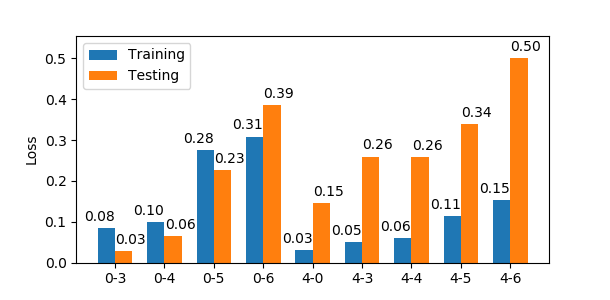
\includegraphics[]{images/conclusion_loss.png}
	% This file was created by matplotlib2tikz v0.7.3.
\begin{tikzpicture}

\definecolor{color0}{rgb}{0.12156862745098,0.466666666666667,0.705882352941177}
\definecolor{color1}{rgb}{1,0.498039215686275,0.0549019607843137}

\begin{axis}[
height=\figureheight,
legend cell align={left},
legend style={at={(0.03,0.97)}, anchor=north west, draw=white!80.0!black},
tick align=outside,
tick pos=left,
width=\figurewidth,
x grid style={white!69.01960784313725!black},
xmin=-0.785, xmax=8.785,
xtick style={color=black},
xtick={0,1,2,3,4,5,6,7,8},
xticklabels={0-3,0-4,0-5,0-6,4-0,4-3,4-4,4-5,4-6},
y grid style={white!69.01960784313725!black},
ylabel={Loss},
ymin=0, ymax=0.52495015965173,
ytick style={color=black},
ytick={0,0.1,0.2,0.3,0.4,0.5,0.6},
yticklabels={0.0,0.1,0.2,0.3,0.4,0.5,}
]
\draw[fill=color0,draw opacity=0] (axis cs:-0.35,0) rectangle (axis cs:0,0.0848326952661315);
\addlegendimage{ybar,ybar legend,fill=color0,draw opacity=0};
\addlegendentry{Training}

\draw[fill=color0,draw opacity=0] (axis cs:0.65,0) rectangle (axis cs:1,0.0985216816457418);
\draw[fill=color0,draw opacity=0] (axis cs:1.65,0) rectangle (axis cs:2,0.275235192127982);
\draw[fill=color0,draw opacity=0] (axis cs:2.65,0) rectangle (axis cs:3,0.308308220500576);
\draw[fill=color0,draw opacity=0] (axis cs:3.65,0) rectangle (axis cs:4,0.0313814810523625);
\draw[fill=color0,draw opacity=0] (axis cs:4.65,0) rectangle (axis cs:5,0.0493501171798515);
\draw[fill=color0,draw opacity=0] (axis cs:5.65,0) rectangle (axis cs:6,0.0601031640727976);
\draw[fill=color0,draw opacity=0] (axis cs:6.65,0) rectangle (axis cs:7,0.114382526963265);
\draw[fill=color0,draw opacity=0] (axis cs:7.65,0) rectangle (axis cs:8,0.152284982224603);
\draw[fill=color1,draw opacity=0] (axis cs:0,0) rectangle (axis cs:0.35,0.0273379426863458);
\addlegendimage{ybar,ybar legend,fill=color1,draw opacity=0};
\addlegendentry{Testing}

\draw[fill=color1,draw opacity=0] (axis cs:1,0) rectangle (axis cs:1.35,0.0646619006853413);
\draw[fill=color1,draw opacity=0] (axis cs:2,0) rectangle (axis cs:2.35,0.226243400408162);
\draw[fill=color1,draw opacity=0] (axis cs:3,0) rectangle (axis cs:3.35,0.385673365935131);
\draw[fill=color1,draw opacity=0] (axis cs:4,0) rectangle (axis cs:4.35,0.145997776799723);
\draw[fill=color1,draw opacity=0] (axis cs:5,0) rectangle (axis cs:5.35,0.259522616167633);
\draw[fill=color1,draw opacity=0] (axis cs:6,0) rectangle (axis cs:6.35,0.257949455544197);
\draw[fill=color1,draw opacity=0] (axis cs:7,0) rectangle (axis cs:7.35,0.339136986151614);
\draw[fill=color1,draw opacity=0] (axis cs:8,0) rectangle (axis cs:8.35,0.499952533001647);
\end{axis}

\end{tikzpicture}
	\caption{Losses of all networks}
	\label{fig:losses}
\end{figure}
\begin{figure}
	\setlength\figureheight{.4\textwidth}
	\setlength\figurewidth{.8\textwidth}
	\centering
	%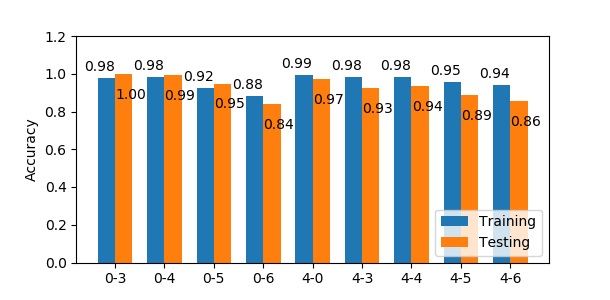
\includegraphics[]{images/conclusion_accuracy.png}
	% This file was created by matplotlib2tikz v0.7.3.
\begin{tikzpicture}

\definecolor{color0}{rgb}{0.12156862745098,0.466666666666667,0.705882352941177}
\definecolor{color1}{rgb}{1,0.498039215686275,0.0549019607843137}

\begin{axis}[
height=\figureheight,
legend cell align={left},
legend style={at={(0.97,0.03)}, anchor=south east, draw=white!80.0!black},
tick align=outside,
tick pos=left,
width=\figurewidth,
x grid style={white!69.01960784313725!black},
xmin=-0.785, xmax=8.785,
xtick style={color=black},
xtick={0,1,2,3,4,5,6,7,8},
xticklabels={0-3,0-4,0-5,0-6,4-0,4-3,4-4,4-5,4-6},
y grid style={white!69.01960784313725!black},
ylabel={Accuracy},
ymin=0, ymax=1.05,
ytick style={color=black},
ytick={0,0.2,0.4,0.6,0.8,1,1.2},
yticklabels={0.0,0.2,0.4,0.6,0.8,1.0,}
]
\draw[fill=color0,draw opacity=0] (axis cs:-0.35,0) rectangle (axis cs:0,0.978448275862069);
\addlegendimage{ybar,ybar legend,fill=color0,draw opacity=0};
\addlegendentry{Training}

\draw[fill=color0,draw opacity=0] (axis cs:0.65,0) rectangle (axis cs:1,0.980769230769231);
\draw[fill=color0,draw opacity=0] (axis cs:1.65,0) rectangle (axis cs:2,0.923469387755102);
\draw[fill=color0,draw opacity=0] (axis cs:2.65,0) rectangle (axis cs:3,0.882902298508019);
\draw[fill=color0,draw opacity=0] (axis cs:3.65,0) rectangle (axis cs:4,0.994047619047619);
\draw[fill=color0,draw opacity=0] (axis cs:4.65,0) rectangle (axis cs:5,0.983870967741935);
\draw[fill=color0,draw opacity=0] (axis cs:5.65,0) rectangle (axis cs:6,0.98030303030303);
\draw[fill=color0,draw opacity=0] (axis cs:6.65,0) rectangle (axis cs:7,0.954710144927536);
\draw[fill=color0,draw opacity=0] (axis cs:7.65,0) rectangle (axis cs:8,0.941028225806452);
\draw[fill=color1,draw opacity=0] (axis cs:0,0) rectangle (axis cs:0.35,1);
\addlegendimage{ybar,ybar legend,fill=color1,draw opacity=0};
\addlegendentry{Testing}

\draw[fill=color1,draw opacity=0] (axis cs:1,0) rectangle (axis cs:1.35,0.990740740740741);
\draw[fill=color1,draw opacity=0] (axis cs:2,0) rectangle (axis cs:2.35,0.948148148148148);
\draw[fill=color1,draw opacity=0] (axis cs:3,0) rectangle (axis cs:3.35,0.839506172839506);
\draw[fill=color1,draw opacity=0] (axis cs:4,0) rectangle (axis cs:4.35,0.972222222222222);
\draw[fill=color1,draw opacity=0] (axis cs:5,0) rectangle (axis cs:5.35,0.925925925925926);
\draw[fill=color1,draw opacity=0] (axis cs:6,0) rectangle (axis cs:6.35,0.935185185185185);
\draw[fill=color1,draw opacity=0] (axis cs:7,0) rectangle (axis cs:7.35,0.888888888888889);
\draw[fill=color1,draw opacity=0] (axis cs:8,0) rectangle (axis cs:8.35,0.856259659969088);
\end{axis}

\end{tikzpicture}
	\caption{Accuracies of all networks}
	\label{fig:accuracies}
\end{figure}
\begin{table}
	\centering
	\caption{Performance of all networks}
	\label{tab:network-performances}
	\begin{tabular}{c|c|c|c|c|c|c|c|c|c}
		& 0-3 & 0-4 & 0-5 & 0-6 & 4-0 & 4-3 & 4-4 & 4-5 & 4-6 \\ \hline
		Train Loss & 0.085 & 0.099 & 0.275 & 0.308 & 0.031 & 0.049 & 0.06 & 0.114 & 0.152 \\
		Test Loss & 0.027 & 0.065 & 0.226 & 0.386 & 0.146 & 0.26 & 0.258 & 0.339 & 0.5 \\ \hline
		Train Accuracy & 0.978 & 0.981 & 0.923 & 0.883 & 0.994 & 0.984 & 0.98 & 0.955 & 0.941 \\
		Test Accuracy & 1.0 & 0.991 & 0.948 & 0.84 & 0.972 & 0.926 & 0.935 & 0.889 & 0.856 \\
	\end{tabular}
\end{table}
\section{Outlook}
\label{sec:discussion-outlook}
The current networks can be improved by tuning the dataset among others.
More lights could be added to the scene or the current light is placed at the position of the camera and points along its view axis directly at the object.
This way more shadows are created in a view presumably leading to detection of more edge features.
For creating optimal faces that are not occluded by others, ray casts for as many vertices in the face as possible need to be performed and checked if the ray hits the actual face.
However, this gets very computationally expensive and would take a huge amount of time.
The advantage of this would be, that those results could be stored an used for finding the second optimal face.
If resources and time are no constraints, every other face could be examined for being the second optimal face.
Its results are then compared with the ones from the first one under the restriction of a given number of views where one should be visible.
Otherwise, choosing a valid face with the maximum distance from the first is a working approach.
In this case, though, a manual deleting of some bad samples needs to be performed.
Furthermore, the trained networks could be tested on real-world samples.
Real-world objects could be digitalized with a 3D scanner and propagated through the network.
This is likely to give somehow different results as true 3D models.
Moreover, real-world colors and materials can be assigned to each model, either CAD or digitalized, for supplying more features.

The networks could be improved by a longer training because no indication of overfitting exists.
Moreover, restarts for the learning rate could be added to avoid the differences in the loss for the four-category networks by stepping over small minima.
Furthermore, a change in a number of groups and their bin size could be evaluated.
However, it cannot be rated if this improves performance.
The minimum of groups should be related to the current number of groups used for the predictions, though.
Probably the largest boost in performance would be a change of the underlying network architecture.
There are many networks that achieve higher accuracies according to the ImageNet challenge in object detection in images like Inception-v4 and ResNet.
If they are combined with the grouping mechanism higher accuracies than with the current implementation are expected.
However, the position of the grouping module and the input of the fully-connected layer for calculating the view discrimination scores are different if the new architecture is nested.
Their properties need to be examined first.


%\appendix			% schaltet Umgebunsvariablen um auf Anhang
%\input{appendix1}		% erster Teil des Anhangs (wird eher selten benötigt)

\backmatter			% Literaturverzeichnis, Index usw.

%%%%%%%%%%%%%%%%%%%%%%%%%%%%%%%%%%%%%%%%%%%%%%%%%
% Literatur
%%%%%%%%%%%%%%%%%%%%%%%%%%%%%%%%%%%%%%%%%%%%%%%%%
\begingroup
\raggedright\sloppy
\bibliography{literature}		% Name der *.bib Datei in der die Literatur steht
\endgroup
%nocite{*}						% Auflisten aller Quellen, auch wenn diese nicht in der Arbeit zitiert sind

% Stil des Literaturverzeichnis (nach DIN1505)
\bibliographystyle{unsrtdin} % sortiert nach Reihenfolge im Text mit Nummern
%\bibliographystyle{plaindin} % alphabetisch sortiert mit Nummer
%\bibliographystyle{alphadin} % alphabetisch sortiert mit Autor-Jahr-Kürzel statt Nummer

\end{document}
